\chapter{Getting Started with Kleene}

\section{Installation and Prerequisites}

\subsection{Pre-compiled Binaries}

This chapter, which is definitely work in progress, is designed to get
you started in Kleene and to give you a quick overview of its capabilities.
The features presented here informally will be treated again with 
more rigor later in the book.

As you read this chapter, it is recommended that you follow along, testing
the examples.  This will, of course, require that you have Kleene and its
prerequisites installed and running on your own computer.  By far the
easiest way to install Kleene is by downloading one of the pre-compiled
binary versions from \url{http://www.kleene-lang.org}.  At the time of
writing, such pre-compiled binaries are available for

\begin{itemize}
\item
Apple OS X, and
\item
Linux
\end{itemize}

\noindent
Check the web site for the latest offerings.  
It is hoped that Kleene will someday be available on Windows.

To install Kleene, you will need to have some basic computer skills, including knowing how
to
download files from the Internet,
launch a terminal application, move around the directory structure,
copy files, edit files, etc.  If this means nothing to you, seek the
help of an expert.

The precompiled binaries have names like \texttt{kleene-mac-0.9.3.5.tar.gz} and
\texttt{kleene-linux-0.9.3.5.tar.gz}; these are sometimes called \emph{tarballs}.  More recent
versions will have higher numbers.  Once downloaded, the tarball should be moved
to a convenient location of your choice, e.g.\@ into directory 
\texttt{\~{}/kleene/}, and then
``unpacked'' with the command

\begin{Verbatim}
$ gunzip kleene-mac-0.9.3.5.tar.gz
\end{Verbatim}

\noindent
This should produce a file named kleene-mac-0.9.3.5.tar,\footnote{Sometimes 
your web browser will \texttt{gunzip} the file for you.} and then ``untar'' that file with

\begin{Verbatim}
$ tar xvf kleene-mac-0.9.3.5.tar
\end{Verbatim}

\noindent
which should produce a directory named \texttt{kleene}.  Inside that directory, 
find a file named \texttt{README.install} and read it carefully, following the 
instructions.  Again, get help as necessary from friends and associates who have 
experience in installing computer
software.

You will also need to have Java 1.5, or a newer version, installed, and
there are various others settings and edits required.  They are all
described in detail in the \texttt{README.install} file.
Corrections, and suggestions for making the installation instructions clearer for all
potential users, would be much appreciated.

\subsection{Compiling Kleene from Source Code}

If a pre-compiled binary works for you, just skip this section and proceed to the next.
You do not need to, and probably do not want to, compile Kleene from the
source code.  ``Building'' Kleene from the source files is currently
rather difficult, an exercise for experts, and this is definitely a target
for simplification in the future.

If a pre-compiled binary does not work for you, and you don't mind a little
challenge, read the files \texttt{README.git} and \texttt{README.build},
which will direct you to download the Kleene source code from a Github
repository.  Follow the instructions in \texttt{README.build} and then
those in \texttt{README.install}.  If you succeed in compiling and running
Kleene in a new operating system, you are urged to contribute the
tarball file for use by others.

\section{Launching the Kleene \acro{gui}}

Once you have followed all the instructions in \texttt{README.install},
you should be able to cd to the directory where the \texttt{Kleene.jar}
file is installed and then invoke 

\begin{Verbatim}
$ java -jar Kleene.jar
\end{Verbatim}

\noindent
or one of the aliases described in \texttt{README.install}.
This should bring up the Kleene \acro{gui} (Graphical User Interface),
which looks like this:


\begin{center}
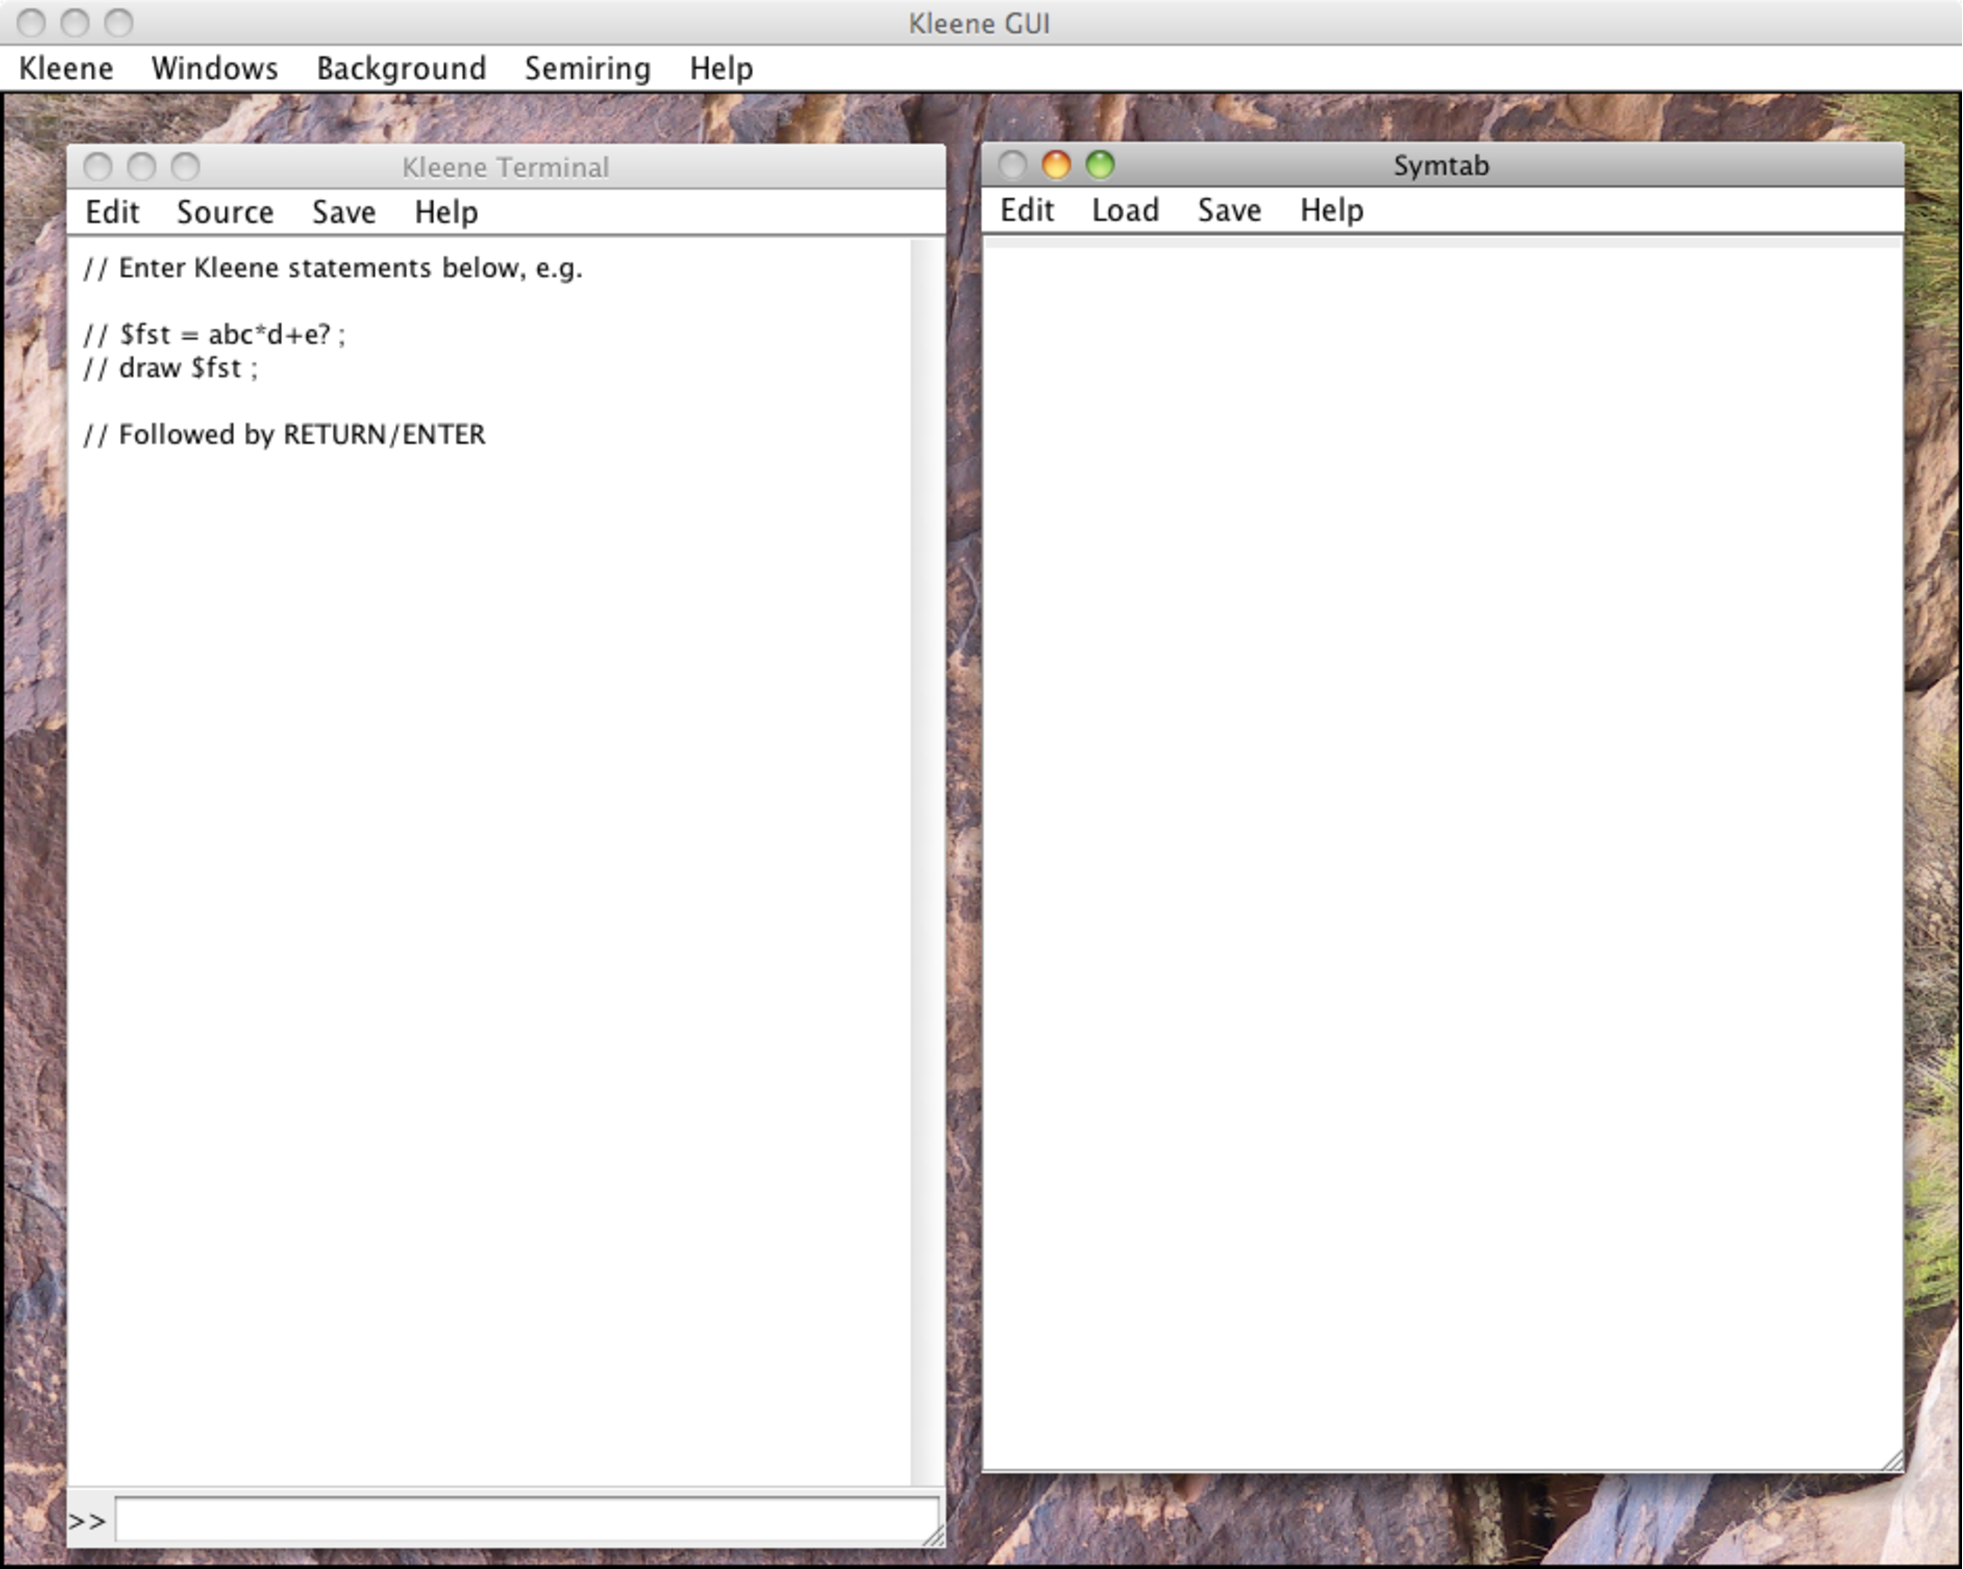
\includegraphics[width=135mm]{images/KleeneGUI.pdf}
%\includegraphics[scale=0.9]{images/<filename>.pdf}
%\includegraphics[width=60mm]{images/<filename>.pdf}
%\includegraphics[height=60mm]{images/<filename>.pdf}
\end{center}


The look-and-feel will be a little different on OS X and Linux.  The
application window, which almost fills the screen, can be minimized using
the buttons at the top.  Inside the application window, there is a
pseudo-terminal window\footnote{It is called a \emph{pseudo} terminal
because it allows you to type commands, and view responses, in a
terminal-like window, but it lacks a history memory and other useful
features of a traditional command-line terminal application.  It is hoped
that this pseudo-terminal can be improved in the future.}  on the left,
and a symbol-table window, initially empty, on the right.  At the very
bottom of the pseudo-terminal window, there is an active one-line text
field where you can enter commands to program (and learn) Kleene
interactively.  

\section{OK, What can you do in Kleene?}

\subsection{First, is it working?}

Just to make sure that Kleene is working, enter the following statement carefully in the bottom line of the
pseudo-terminal window:

\begin{Verbatim}
$fsm = dog | cat | bird ;
\end{Verbatim}

\noindent
Be sure to include the semicolon at the end, and press the Enter key on your keyboard to
initiate interpretation.  If everything is working, you should see an icon named
\verb!$fsm!
appear in the symbol-table window on the right.  Your statement has 
been successfully interpreted to
build a finite-state machine.  In this case, it is an \fsm{} that encodes the
language that contains just three words:  ``dog,'' ``cat'' and ``bird.''

\subsection{Visualizing Finite-State Machines}

To view the finite-state machine that you just created, you can right-click on the \verb!$fsm! icon and
select the drop-down-menu item
named \texttt{draw}.  Equivalently, you can enter 


\begin{Verbatim}
draw $fsm ;
\end{Verbatim}

\noindent
manually in the pseudo-terminal.  In fact, selecting the \texttt{draw} menu
item causes the statement \verb!draw $fsm ;! to be written in the
pseudo-terminal, and then interpreted, exactly as if you had typed it yourself.  This
behavior is designed to help you learn the scripting language.

If everything is working correctly, you should see the following \fsm{}
diagram appear on your screen.


\begin{center}
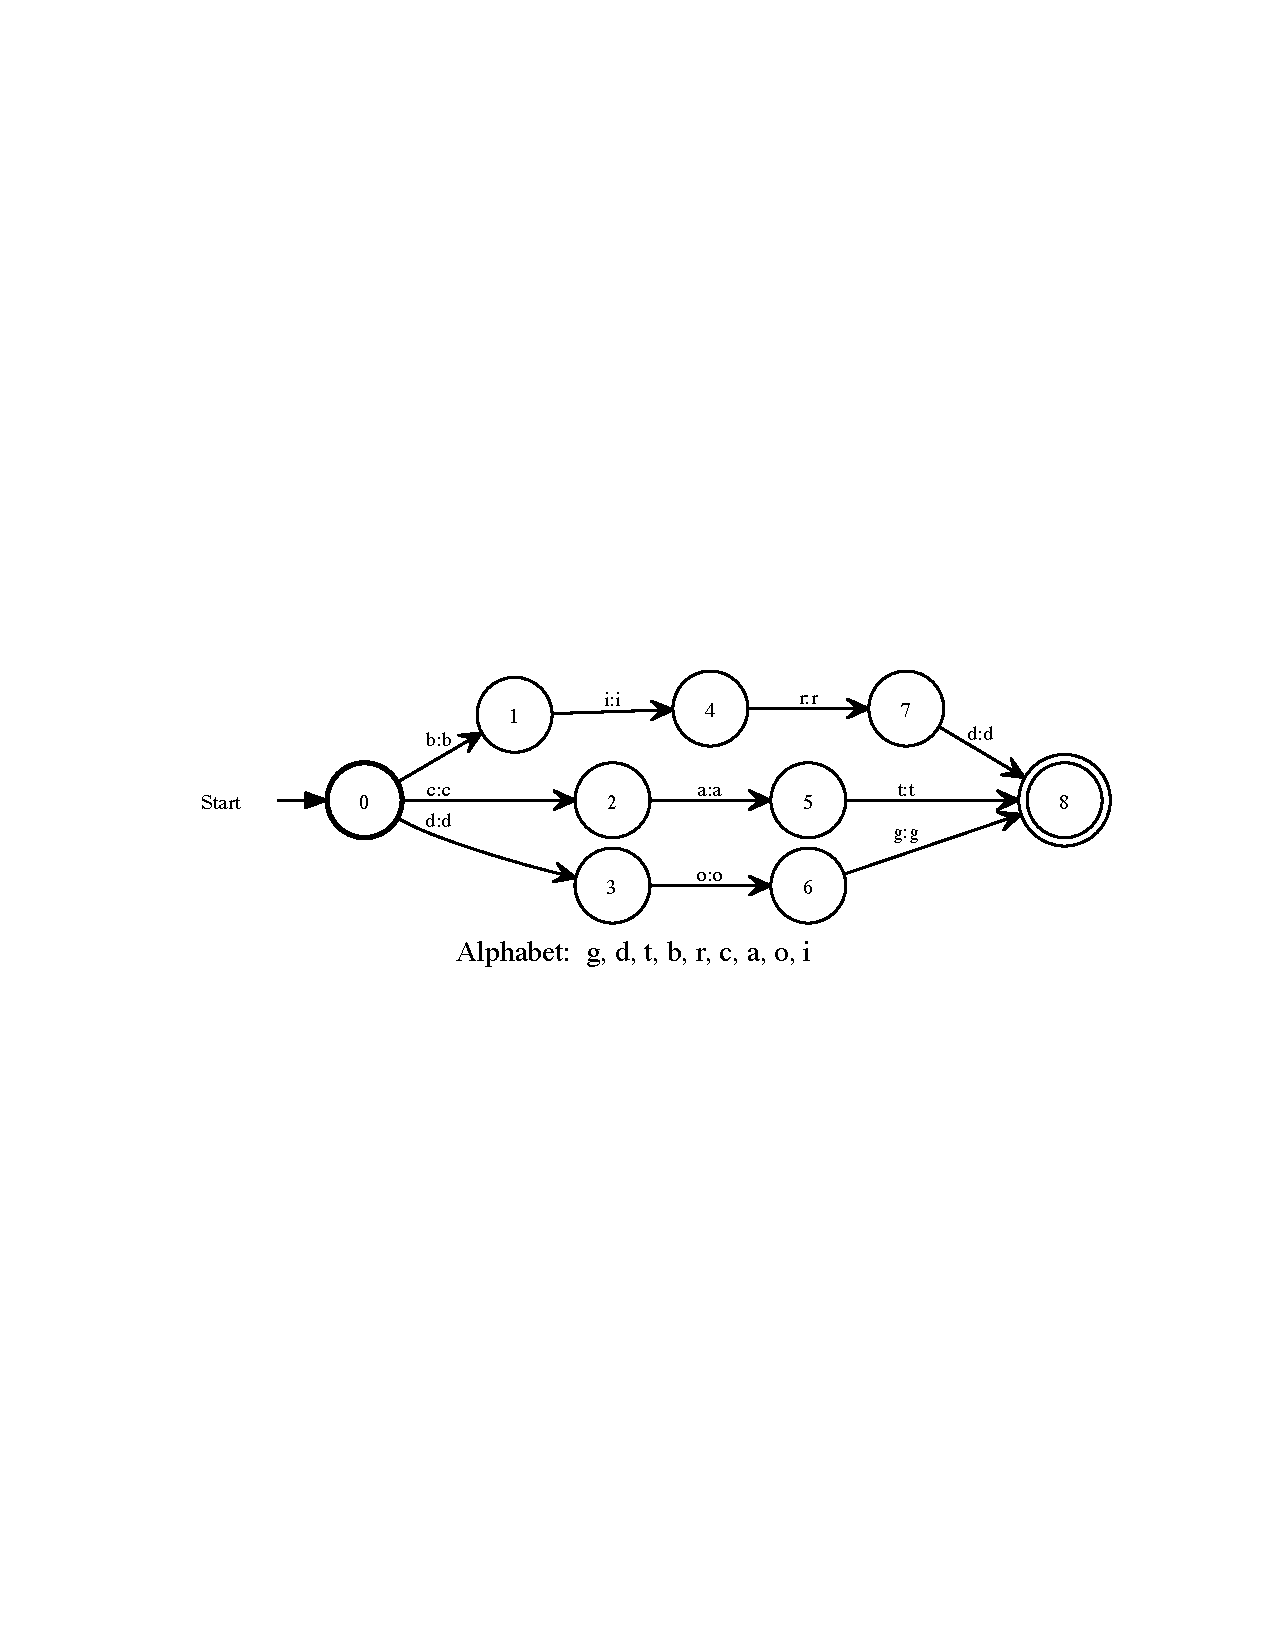
\includegraphics[width=135mm]{images/dogcatbird.pdf}
%\includegraphics[scale=0.9]{images/<filename>.pdf}
%\includegraphics[width=60mm]{images/<filename>.pdf}
%\includegraphics[height=60mm]{images/<filename>.pdf}
\end{center}


Note that the finite state machine (\init{fsm}) has a start state, represented by a bold
circle labeled ``Start,'' a single final state represented with a double circle, and
other states
represented with plain circles.  Where the \fsm{} has \texttt{n} states, they are
numbered in a dense range from \texttt{0} to \texttt{n - 1}.  The start state is
often, but not always, number \texttt{0}.   This particular \fsm{} has three \emph{paths} leading from the
start state to the final state, each path encoding one word.

Each transition or \emph{arc} leading from a state to a
state has a label like \texttt{d:d}.  The first \texttt{d} is termed the \emph{input
symbol}, and the second the \emph{output symbol}, in the OpenFst visualization of
\init{fsm}s.  Thus the compound labels are always interpreted as
\texttt{InputLabel}:\texttt{OutputLabel}.

In other traditions, \init{fsm}s are visualized a bit differently, and
the terminologies
vary, sometimes confusingly.  A label like \texttt{d:d} could be thought of as
\texttt{LeftSymbol}:\texttt{RightSymbol}.  In the Two-Level-Morphology tradition,
\fsm{}s are usually  visualized vertically, with upper-side symbols
called \emph{lexical} symbols, because they matched symbols in a lexicon, and
with lower-side symbols called \emph{surface} symbols, because they matched
symbols in surface strings: \texttt{Lexical}:\texttt{Surface}.  

The Xerox/\acro{parc} tradition also visualizes \fsm{}s vertically but
emphasizes the bi-directionality of
transducers: either side could be \emph{used} as the input side, and so the opposite
of the side currently being used as the input side is the output side.  
Abstracting away from how a
particular \fsm{} is being used, Xerox researchers often refer to
the labels as \emph{upper} and \emph{lower}:  \texttt{Upper}:\texttt{Lower}.  

Kleene is based on the OpenFst library, but with some powerful semantic features
borrowed from
the Xerox tradition.  In this book, it is sometimes important to
understand an \fsm{} in OpenFst terms, as having \texttt{Input}:\texttt{Output}
labels.  At other times, where the bi-directionality of \fsm{}s is
relevant, I will talk about \texttt{Upper}:\texttt{Lower} labels. 

The ``sides'' or ``levels'' of an \fsm{} are technically known as \emph{projections}, and we will 
refer to the input and output projections when thinking in OpenFst terms, and we will
refer to the upper and lower projections when thinking in Xerox terms.

\subsection{Compile regular expressions into \fsm{}s}

\subsubsection{Assignment Statements}

The example that we used previously for testing

\begin{Verbatim}
$fsm = dog|cat|bird ;
\end{Verbatim}

\noindent
is an assignment statement that has a variable \verb!$fsm! on the left-hand side and a
\emph{regular expression} on the right-hand side, all terminated with a semicolon.  Such
a statement can continue over multiple lines.

Many programmers will already have experience with programming languages, such as Perl,
Python and Java, that support a kind of regular expressions to
perform various useful tasks, including pattern matching and tokenization.  While these
Perl-like regular expressions are often very useful, they are not always \emph{regular}
in the mathematical sense, and so they don't have all the attractive properties of truly
regular expressions.\footnote{For a thorough presentation of ``regular'' expressions as
they appear in common programming languages and operating-system utilities, see the book \emph{Mastering Regular Expressions} by
\citet{friedl:2006}.}

In contrast to programming-language ``regular'' expressions, the regular expressions of Kleene are true regular
expressions in the sense that they always
encode \emph{regular languages} or \emph{regular relations}, and they compile into
finite-state machines (\fsm{}s).  Such regular languages/relations, and the
corresponding \fsm{}s, have mathematically clean and powerful \emph{closure properties}, meaning
that they can be combined together using various operations---including concatenation,
union and composition---and the results are still \emph{regular}.  These terms will be explained as we progress.


\subsubsection{Regular Expressions by Example}

We will look in detail at Kleene regular expressions in the next chapter.  
For now, let's look at some simple examples to get an
intuitive feel for regular expressions and the \fsm{}s corresponding to them.  One of the simplest regular
expressions consists of just a single letter, e.g. \texttt{d}.  Try entering the
following in the Kleene \acro{gui}.

\begin{Verbatim}
$fsm = d ;
draw $fsm ;
\end{Verbatim}

\noindent
The resulting \fsm{} has two states, one the start state and the other a final state,
with one arc labeled \texttt{d:d} leading from the start state to the final state.  


\begin{center}
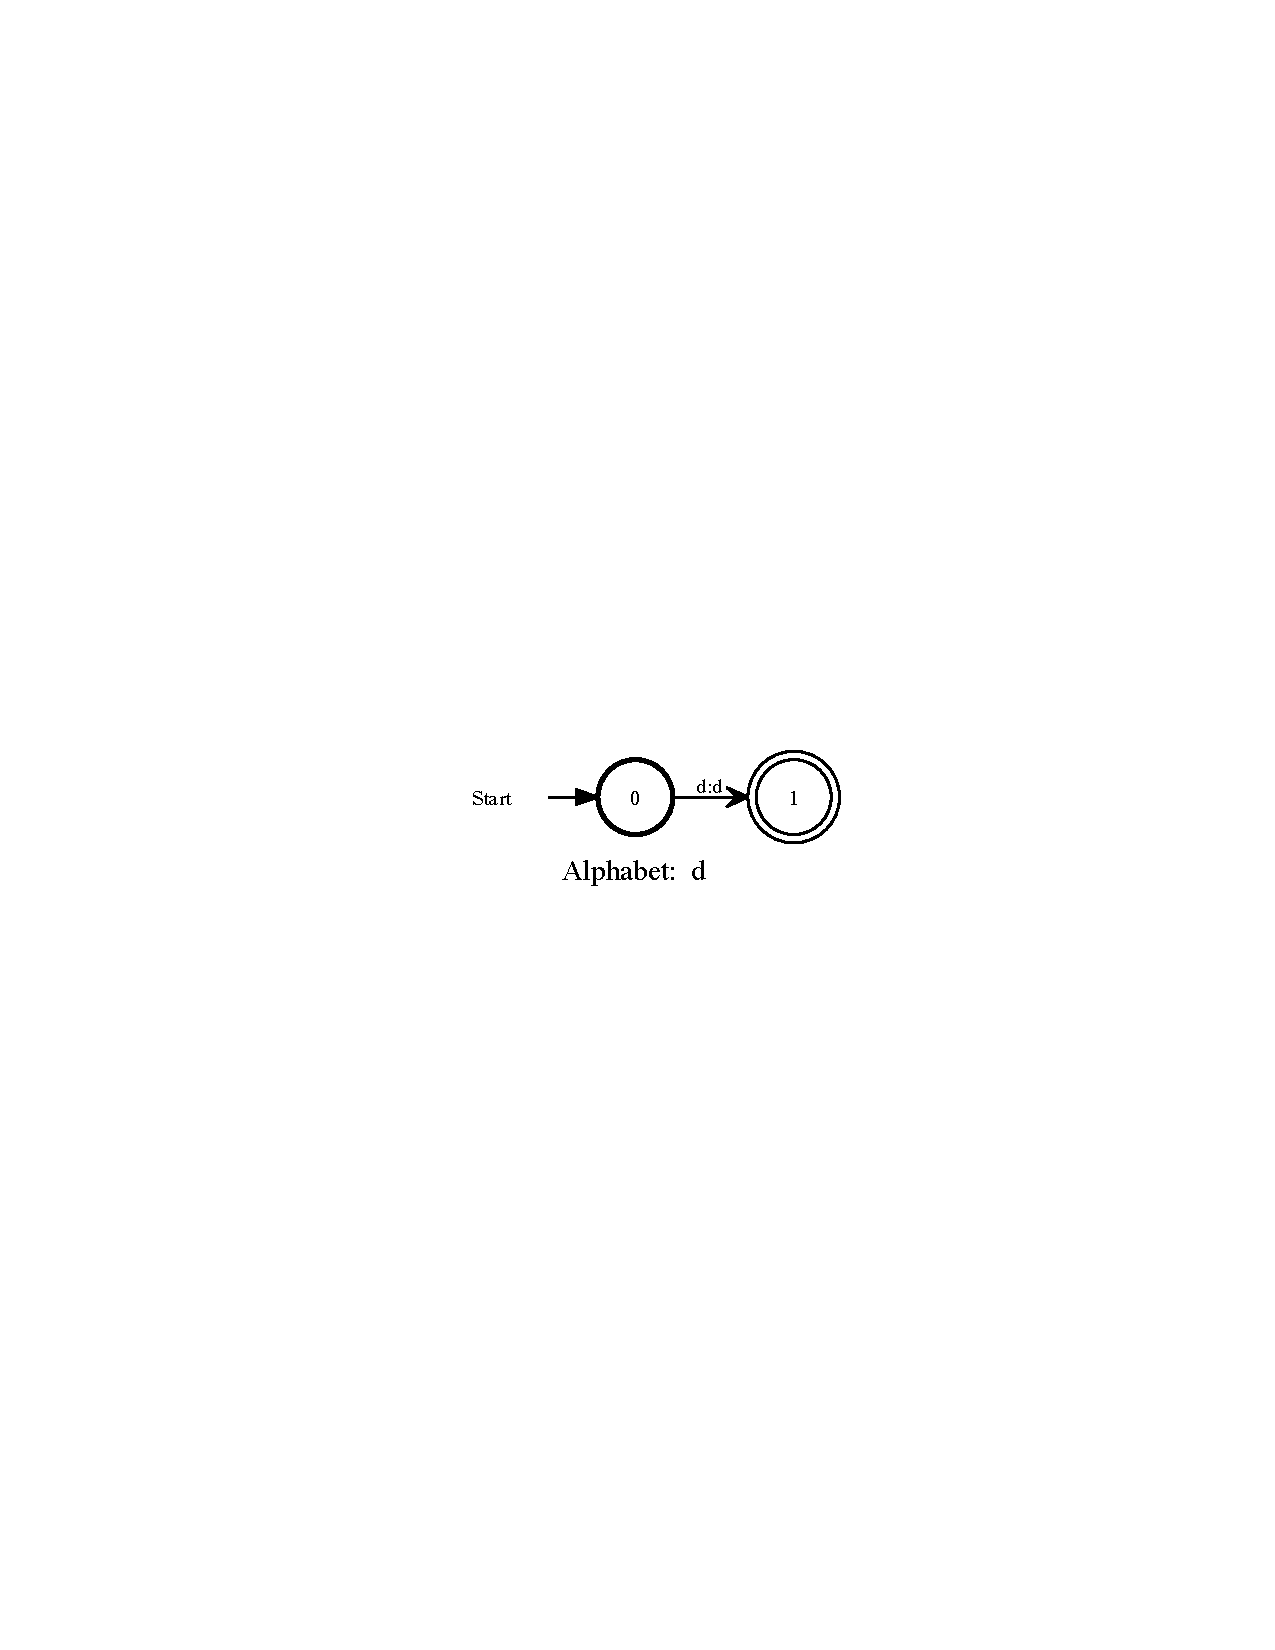
\includegraphics{images/d.pdf}
%\includegraphics[scale=0.9]{images/<filename>.pdf}
%\includegraphics[width=60mm]{images/<filename>.pdf}
%\includegraphics[height=60mm]{images/<filename>.pdf}
\end{center}

\noindent
The regular expression \texttt{d} describes the regular language consisting of just the
one string ``d.''  The \fsm{} \emph{encodes} this language, which means that if you
\emph{apply} it to the string ``d,'' it will match and \emph{accept} it, and it will reject all other
strings, including ``a,'' ``z,'' ``dog,'' ''mmmmmm,'' ``hwiughuiegw,'' etc.  An \fsm{}
can thus be used as an \emph{acceptor} that accepts all and only the strings in the
language that it encodes.

This same \fsm{} can be viewed as an \emph{identity transducer} that maps the string
``d'' to ``d,'' i.e.\@ maps ``d'' to itself.  In OpenFst, the labels on the arcs are always
two-level, \texttt{input}:\texttt{output}, or, in the Xerox visualization,
\texttt{upper}:\texttt{lower}.  An \fsm{} like that above is interpreted either as an acceptor
or as an identity transducer, depending on what is needed by an operation.

In the Kleene \acro{gui}, you can actually test an \fsm{}, to see what it accepts and rejects, by entering

\begin{Verbatim}
test $fsm ;
\end{Verbatim}

\noindent
This will bring up a test window into which you can type an input string.


\begin{center}
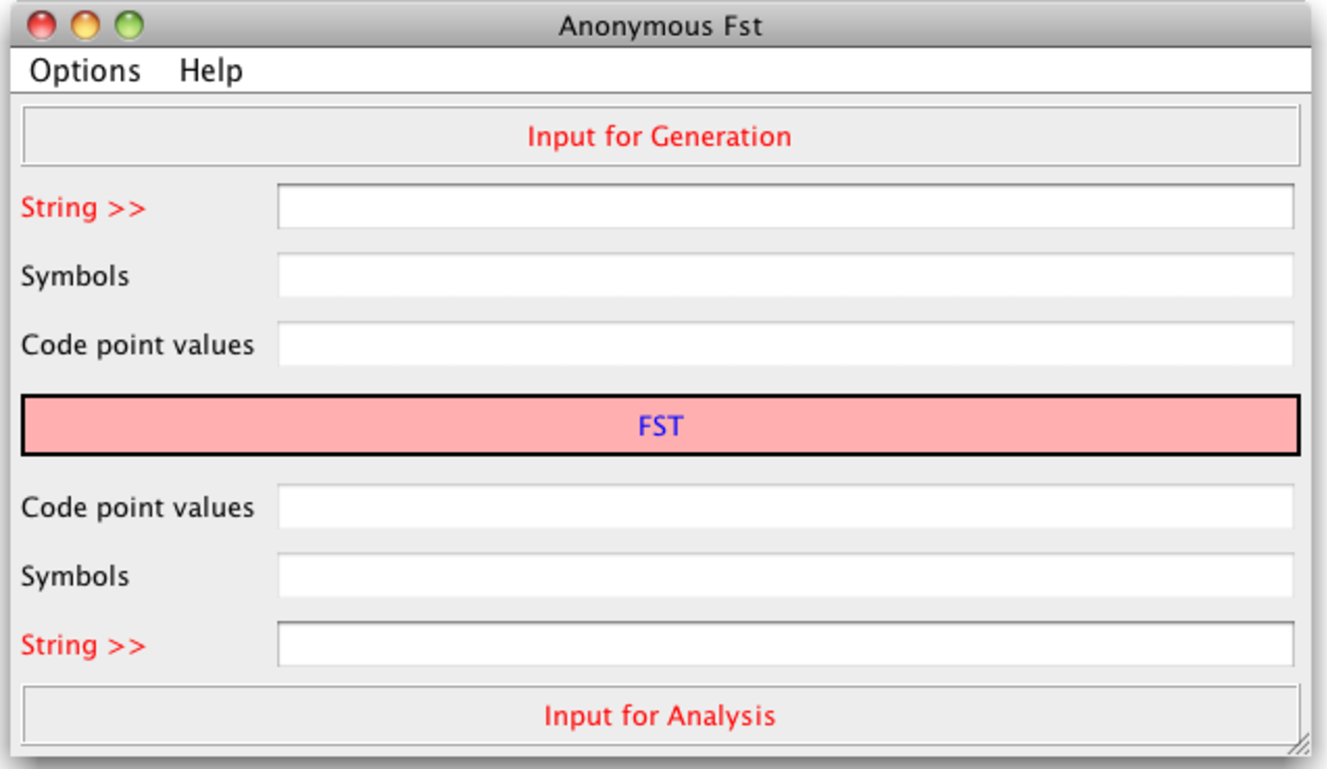
\includegraphics[width=135mm]{images/testWindow.pdf}
%\includegraphics[scale=0.9]{images/<filename>.pdf}
%\includegraphics[width=60mm]{images/<filename>.pdf}
%\includegraphics[height=60mm]{images/<filename>.pdf}
\end{center}

\noindent
The \fst{} being tested
is represented by the bar labeled ``FST'' in the center.
The test window has two string-input fields, one at the top and one at the bottom, both labeled
``String>>.''  For testing
an acceptor, it doesn't matter which field you use.  If you enter \texttt{d} in the top 
field, and then press the Enter key, the answer 


\begin{Verbatim}
d: 0.0
\end{Verbatim}

\noindent
will appear in the history part
of the pseudo-terminal window.  This indicates that the input string was accepted
by the \fsm{}.  (Don't worry now
about the ``0:0,'' which is a weight and will be explained later.)
You get the same result if you enter \texttt{d} in the
lower-side input window.  But if you enter any other string, such as ``b'' or
``dd'' or ``ant'' or ``elephant,'' a message
indicates that the output is empty, i.e.\@ that the input string was not
accepted.

Now let's look at a slightly more complicated regular expression

\begin{Verbatim}
$fsm = dog ;
draw $fsm ;
\end{Verbatim}

\noindent
that involves the \emph{concatenation} of three characters: \texttt{d} followed by
\texttt{o} followed by \texttt{g}.   In Kleene regular expressions, there is no
explicit operator for concatenation; you just type one symbol after another---or
more generally, one operand after another---and they will be concatenated.  
The argument to the \texttt{draw} command can be
an arbitrarily complex regular expression, so one could alternatively just enter

\begin{Verbatim}
draw dog ;
\end{Verbatim}

The \fsm{} that encodes this language, consisting
of the one string ``dog,'' has four states and tree arcs.

\begin{center}
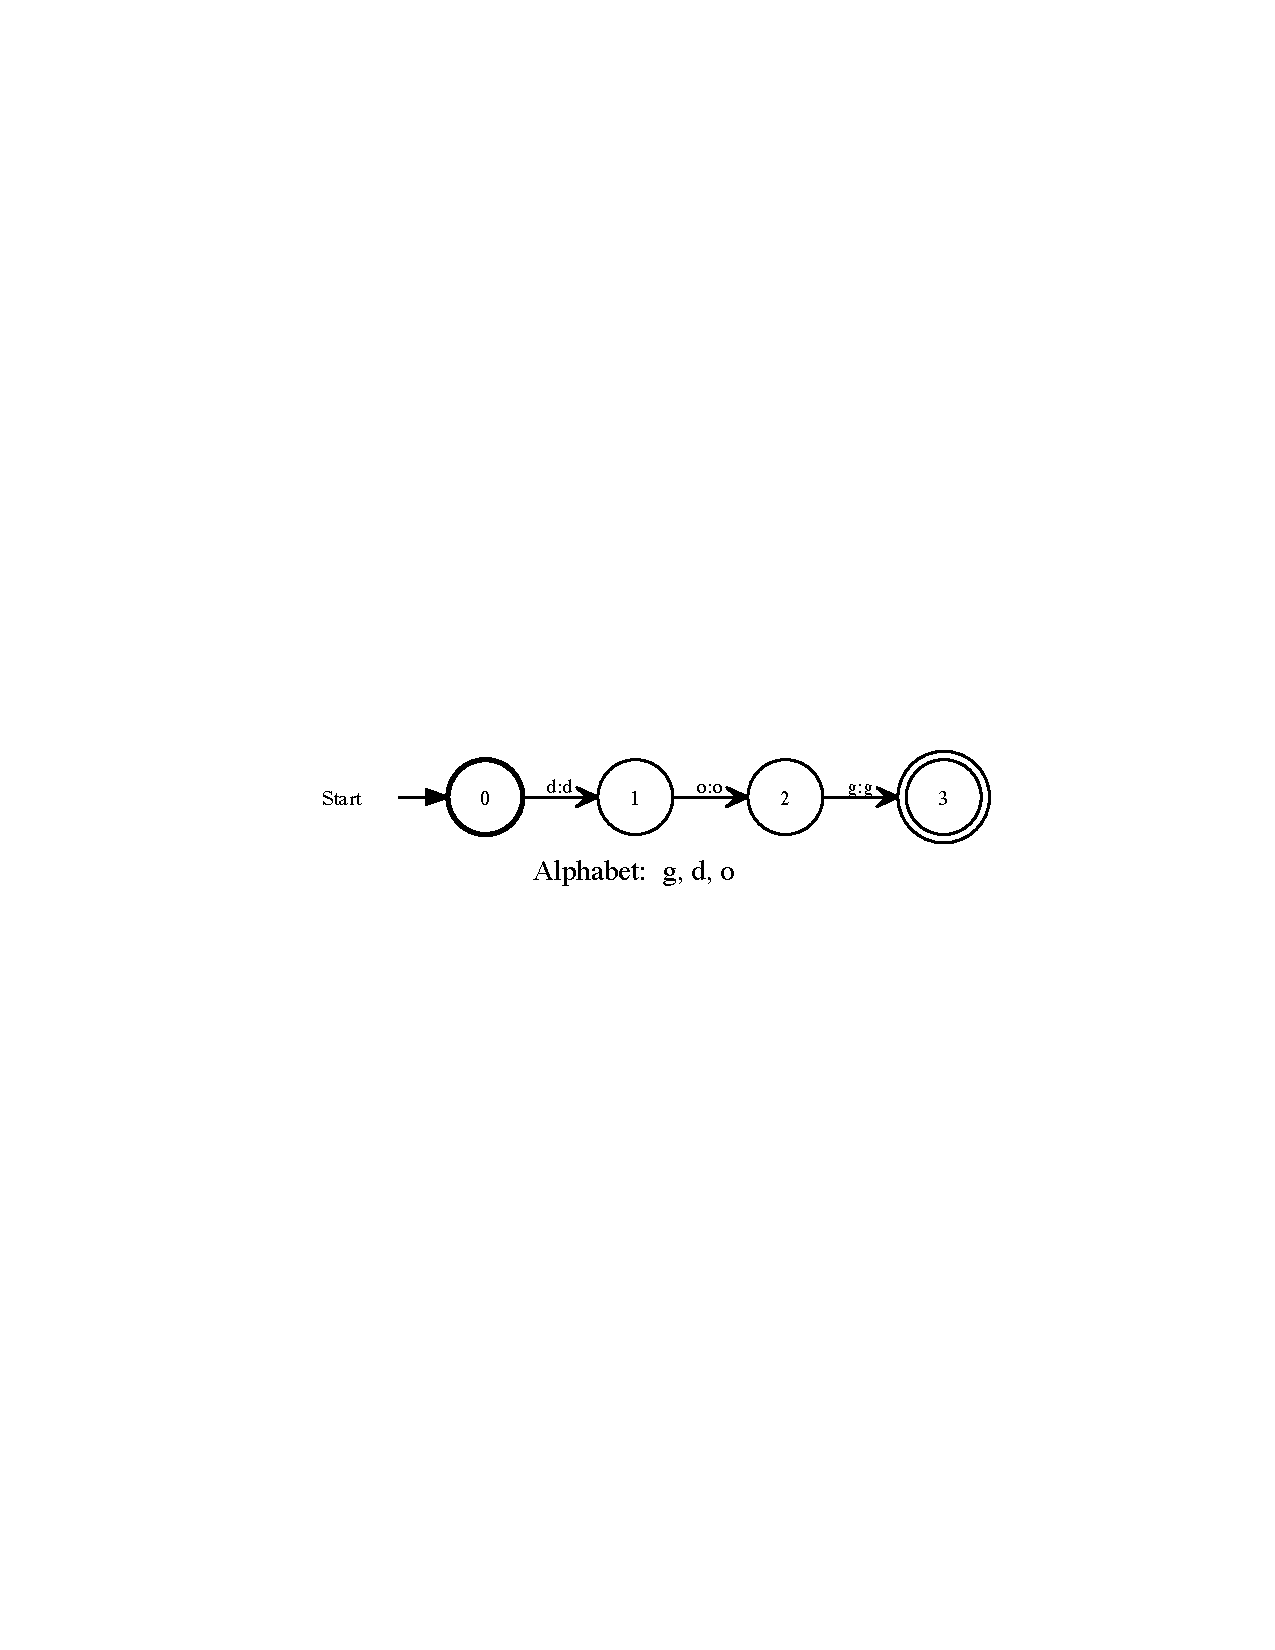
\includegraphics{images/dog.pdf}
%\includegraphics[scale=0.9]{images/<filename>.pdf}
%\includegraphics[width=60mm]{images/<filename>.pdf}
%\includegraphics[height=60mm]{images/<filename>.pdf}
\end{center}

The testing procedure that \emph{applies} this \fsm{} to the string ``dog,'' involves
first setting a match pointer to the first character \texttt{d} in the input string, 
initializing the machine in
its start state, and then looking for an arc labeled \texttt{d} leading out of the
start state.  There is such an arc in this example, so the application 
\emph{consumes} the input symbol \texttt{d}, resets the match pointer to the next
symbol \texttt{o}, and resets
the machine to state 1,
which is the destination state of the arc labeled \texttt{d}.
The current
state of the machine is now state 1.  From the current state, the
process continues, matching and consuming the \texttt{o}, and putting the machine in
state two; then matching and consuming the \texttt{g}, leaving the machine in state 3.
Because state 3 is a final state (indicated by the double circle), and because the input 
string is fully consumed (no input symbols are left over), the
application is a success, and the finite-state machine matches and \emph{accepts} the input string
``dog.''  If this machine were applied to any other input string, it would fail to match, and the
string would be rejected.   

Note that a finite-state machine (\fsm{}) has a finite number of states---though there
might be hundreds of thousands or even millions of them---and there is no other memory
mechanism, such as a stack, used during application.  At any given time during
application, a finite-state machine is in exactly one of its finite number of states.
And when a machine is in a particular state, the only thing that affects its
progression
to the next state is the next input symbol; it has no stack or other memory to
influence where it goes next.

Now let's try a slightly more complicated regular expression, involving both
concatenation and union, for which the operator is the vertical bar \verb!|!. 

\begin{Verbatim}
$fsm = dog|cat|bird|horse ;
draw $fsm ;
\end{Verbatim}

\noindent
For improved readability, you can insert spaces and newlines as desired, e.g.

\begin{Verbatim}
$fsm = dog
    |  cat
    |  bird
    |  horse ;
draw $fsm ;
\end{Verbatim}

\noindent
The resulting \fsm{} encodes the language of four words---``dog,'' ``cat,'' ``bird''
and ``horse''---and clearly has four \emph{paths} leading from the start state to the
final state.


\begin{center}
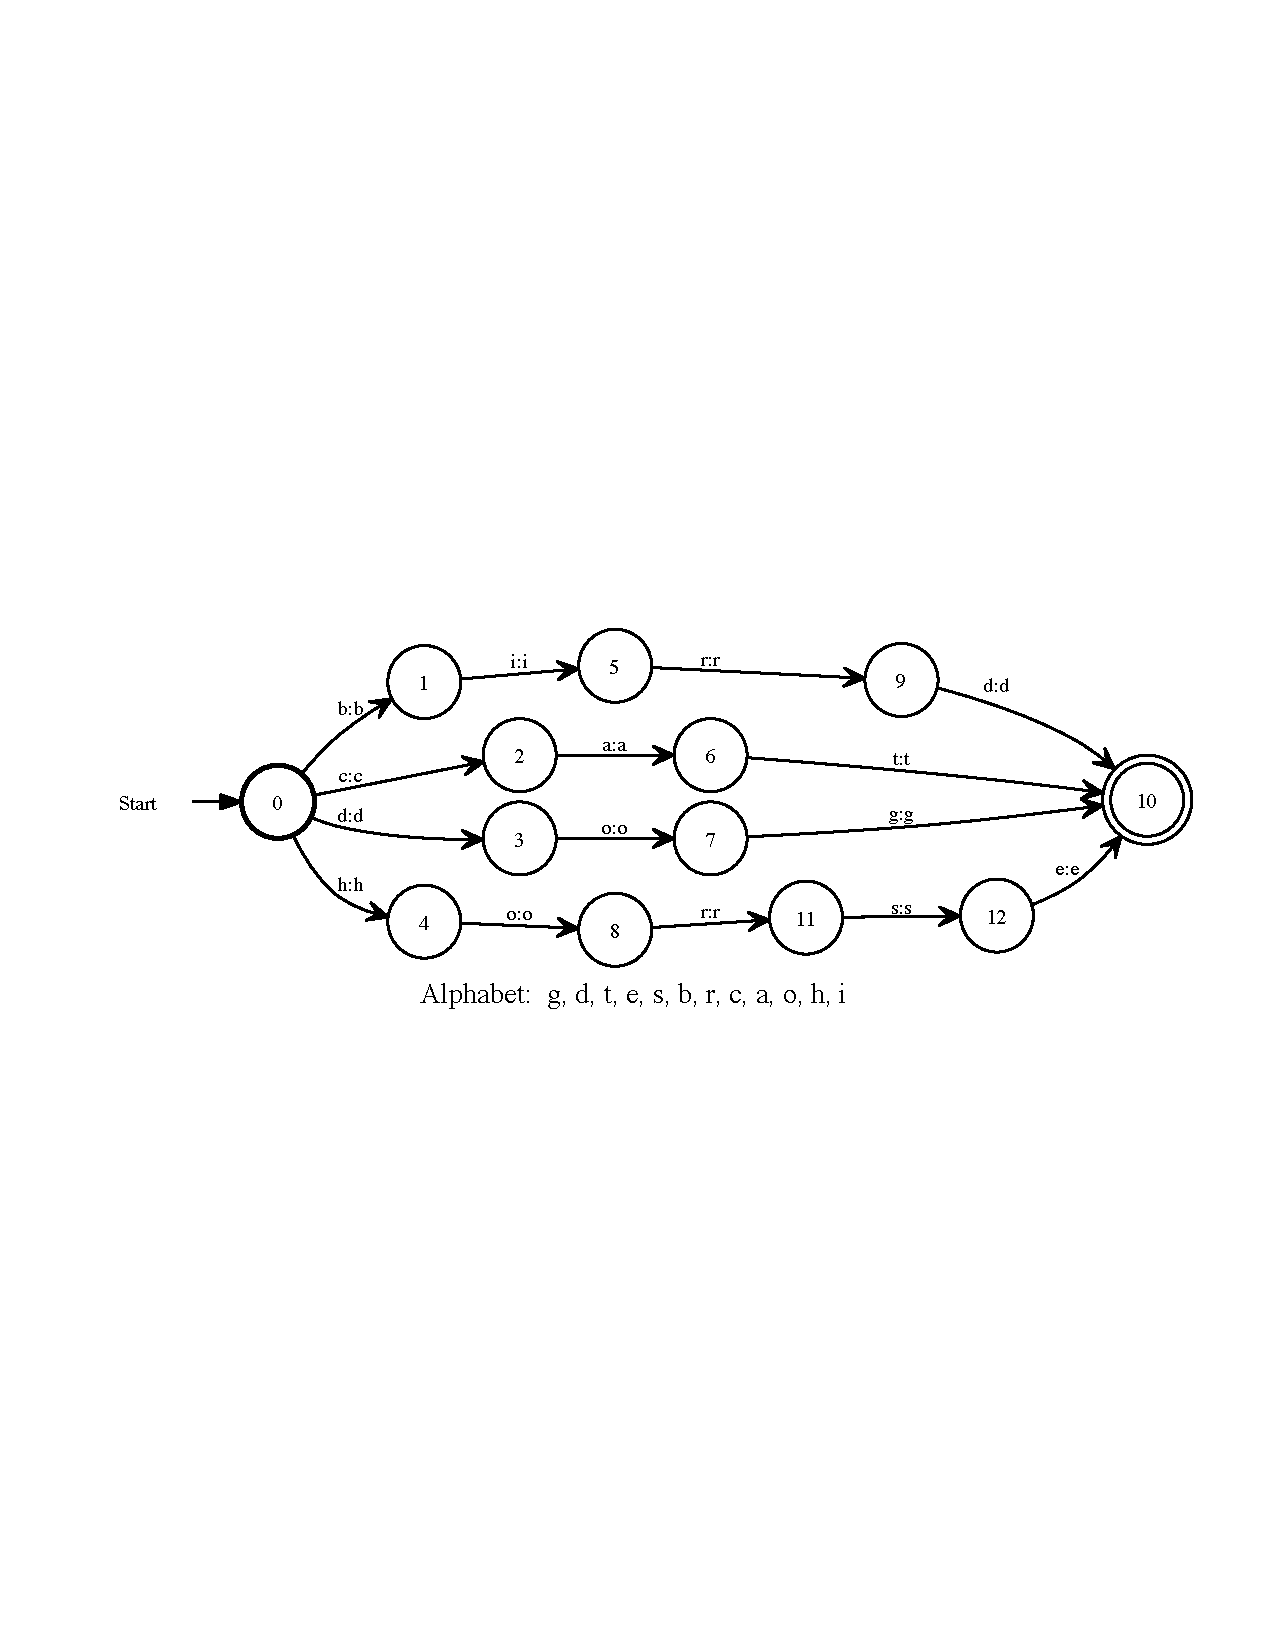
\includegraphics[width=135mm]{images/dogcatbirdhorse.pdf}
%\includegraphics[scale=0.9]{images/<filename>.pdf}
%\includegraphics[width=60mm]{images/<filename>.pdf}
%\includegraphics[height=60mm]{images/<filename>.pdf}
\end{center}

\noindent
If you test this \fsm{}, 

\begin{Verbatim}
test $fsm ;
\end{Verbatim}

\noindent
you will find that it accept the four strings, and no others.

When the \fsm{} is an acceptor, the \texttt{print} command will list the strings:

\begin{Verbatim}
print $fsm ;
// outputs:  dog cat bird horse
print Hello ;
// outputs:  Hello
print apple | orange | banana| fig | cherry ;
// outputs:  apple orange banana fig cherry
\end{Verbatim}

\noindent
Note that a language is a set of strings, and in a set, the order is
insignificant.  \fsm{}s may be constructed, and words encoded by the \fsm{}
may be printed, in orders that you didn't expect.

In general, spaces and other whitespace characters are ignored in Kleene regular
expressions unless they are explicitly literalized.  
One way to literalize spaces, and other
special characters, is to precede them with the backslash character \textbackslash.

\begin{Verbatim}
// This is a comment:
// Printing a string with a literal space
print Hello\ world ;
// outputs:  Hello world (as a single string)
\end{Verbatim}

\noindent
Another equivalent way to literalize a space is to put it inside double quotes:

\begin{Verbatim}
print Hello " " world ;
// or
print "Hello world" ;
draw "Hello world" ;
\end{Verbatim}

Kleene regular expressions, like Perl regular expressions, can also use parentheses for
grouping, a postfixed asterisk * meaning zero or more, a postfixed plus-sign +,
meaning one or more, and a postfixed question mark ? indicating that the preceding
expression is optional.  The following example encodes the words ``dog,'' ``cat'' and
``horse,'' each with an optional \texttt{s} on the end, for a total of six strings.

\begin{Verbatim}
$fsm = ( dog | cat | horse ) s? ;
print $fsm ;
// outputs:  dog dogs cat cats horse horses
\end{Verbatim}

\noindent
And this next example encodes the language of all strings that start with zero or more
\texttt{a} letters, followed by one or more \texttt{b} letters, followed by a
\texttt{c}, \texttt{d}, \texttt{e} or \texttt{f}, and ending with an optional
\texttt{g}.

\begin{Verbatim}
$fsm = a*b+(c|d|e|f)g? ;
\end{Verbatim}

\noindent
This language is infinite in size but still regular, and it is
encoded in a compact \fsm{}.


\begin{center}
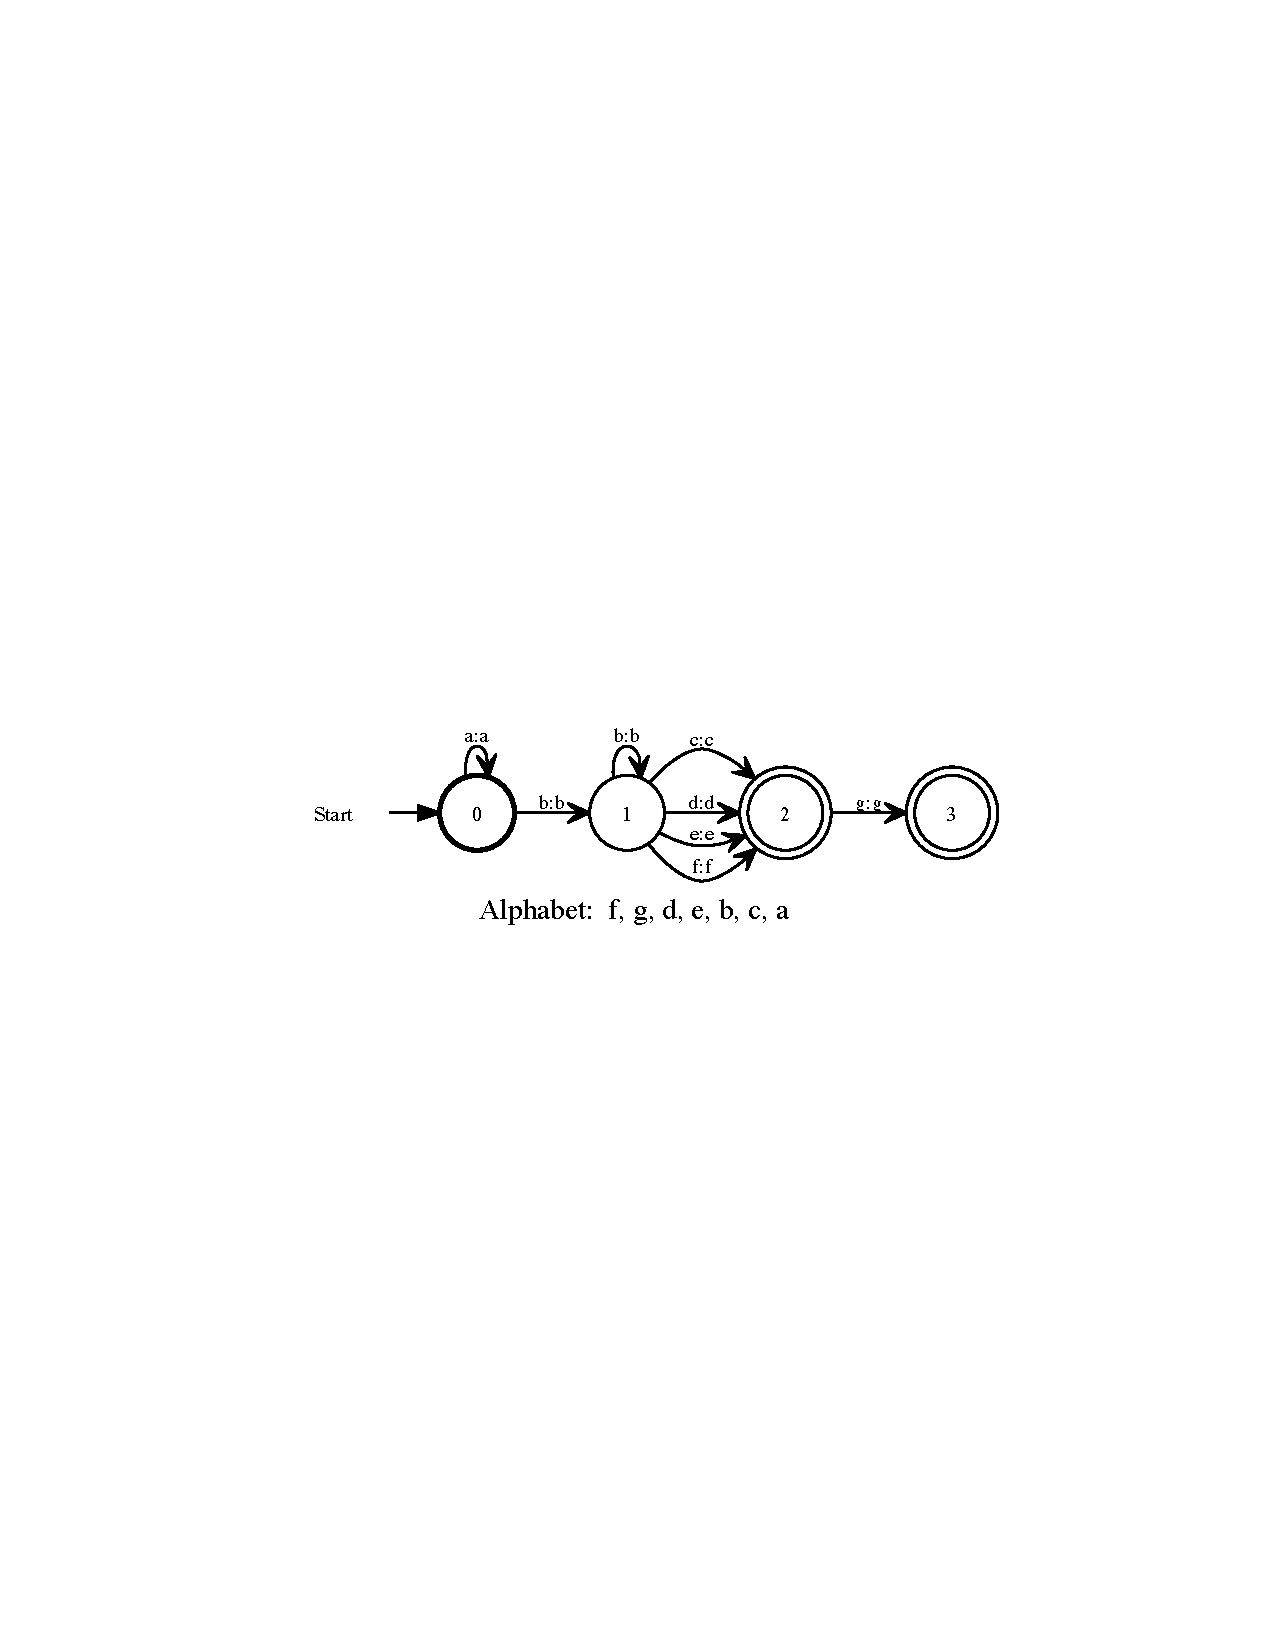
\includegraphics{images/infin.pdf}
%\includegraphics[scale=0.9]{images/<filename>.pdf}
%\includegraphics[width=60mm]{images/<filename>.pdf}
%\includegraphics[height=60mm]{images/<filename>.pdf}
\end{center}

When it becomes tedious to type long unions of symbols, e.g.
\texttt{(a|b|c|d|}\ldots{}\texttt{x|y|z)} one can
use the Perl-like square-bracketed notation for character unions: for
example, \texttt{[a-z]} encodes the union of all characters starting at
\texttt{a} and ending with \texttt{z}.  Similarly, \texttt[aeiou] denotes
the union of \texttt{a}, \texttt{e}, \texttt{i}, \texttt{o} and \texttt{u}.


\begin{Verbatim}
// Three equivalent regular expressions
$fsm1 = a*b+(c|d|e|f)g? ;
$fsm2 = a*b+[cdef]g? ;
$fsm3 = a*b+[c-f]g? ;
\end{Verbatim}

\noindent
The following example encodes the language of all strings that start with an English
alphabet letter, uppercase or lowercase, and then continues with zero or more alphabetic letters or digits:

\begin{Verbatim}
$fsm = [A-Za-z][A-Za-z0-9]* ;
\end{Verbatim}

\noindent
The resulting \fsm{} will accept strings like ``Apple,'' ``a27,'' ``dOg,''
``z3b4n6'' and
``d2T456m7'' while rejecting strings such as ``4abc'' and ``26.''

Regular languages can be subtracted from each other:

\begin{Verbatim}
$lang = (dog | cat | elephant | apple | orange) - 
           (banana | apple | orange) ;
print $lang ;
// outputs: dog cat elephant
\end{Verbatim}

\noindent
Here, the resulting \fsm{} encodes the language consisting of the strings ``dog,'' ``cat'' and ``elephant.''
It is \emph{not} necessary to put spaces around the vertical-bar operator |.
As already stated, white space is ignored in Kleene regular expressions
unless it is explicitly literalized.

Regular languages can also be intersected, resulting in a new language
containing all and only the strings they have in common.
The operator for intersection is \&.

\begin{Verbatim}
$commonAnimals = 
   (dog | cat | elephant | whale | ant | bird | reindeer) & 
   ( cat | horse | reindeer | snail | whale ) ; 
print $animals ;
// outputs: cat whale reindeer
\end{Verbatim}

The . (dot) represents \emph{any} symbol, so the \fsm{} resulting from the
assignment statement

\begin{Verbatim}
$fsm = p . t ;
\end{Verbatim}

\noindent
accepts words including ``pat,'' ``pet,'' ``pit,'' ``pot'',
``put,'' ``pbt,'' ``ppt,'' etc.  And because . really 
represents any symbol, the expression
\verb!.*! represents the Universal Language, the language that contains all possible
strings of any character, of any length, including the empty (zero-length) string.

\begin{Verbatim}
$UnivLang = .* ;
\end{Verbatim}

\noindent
Note that in Kleene, as in the Xerox Finite State Toolkit, is it not necessary
for the programmer to declare the alphabet being used.  In Kleene regular
expressions, the . really represents any possible symbol.

The Empty Language is the language that contains no strings at all, not even the empty
string.  There are an infinite number of ways to denote the Empty Language, including

\begin{Verbatim}
$EmptyLang = .* - .* ;   // Universal Language minus itself
$EmptyLang = dog - dog ; // one-string language minus itself
\end{Verbatim}

\noindent
and

\begin{Verbatim}
$EmptyLang = ~.* ;
\end{Verbatim}

\noindent
where \~{} is the \emph{complement} operator, returning the language of all possible
strings, i.e.\@ the Universal Language, except
(i.e.\@ minus) the strings in the language it applies to.  Thus \texttt{\~{}.*} is
equivalent to \texttt{.* - .*}, the Universal Language minus itself.

The empty string is the string of zero length, containing no symbols at all.  It can be
notated in Kleene as \verb!""!.  The Empty String Language, not to be confused with the Empty
Language, is the language that contains exactly one string, the empty string.

\begin{Verbatim}
$EmptyStringLang = "" ;
\end{Verbatim}

\subsection{Optimization of \fsm{}s}

When \fsm{}s are built in Kleene, they are automatically \emph{optimized}, which involves a
combination of determinization, minimization and epsilon-removal.  The epsilon, which can be
denoted as \verb!""! in regular expressions, is the empty
(zero-length) string, and epsilon-removal involves the
elimination of all arcs that have [eps]:[eps] labels.  Thus the assignment


\begin{Verbatim}
$fsm = a "" c ;
\end{Verbatim}

\noindent
creates a network that initially looks like 

\begin{center}
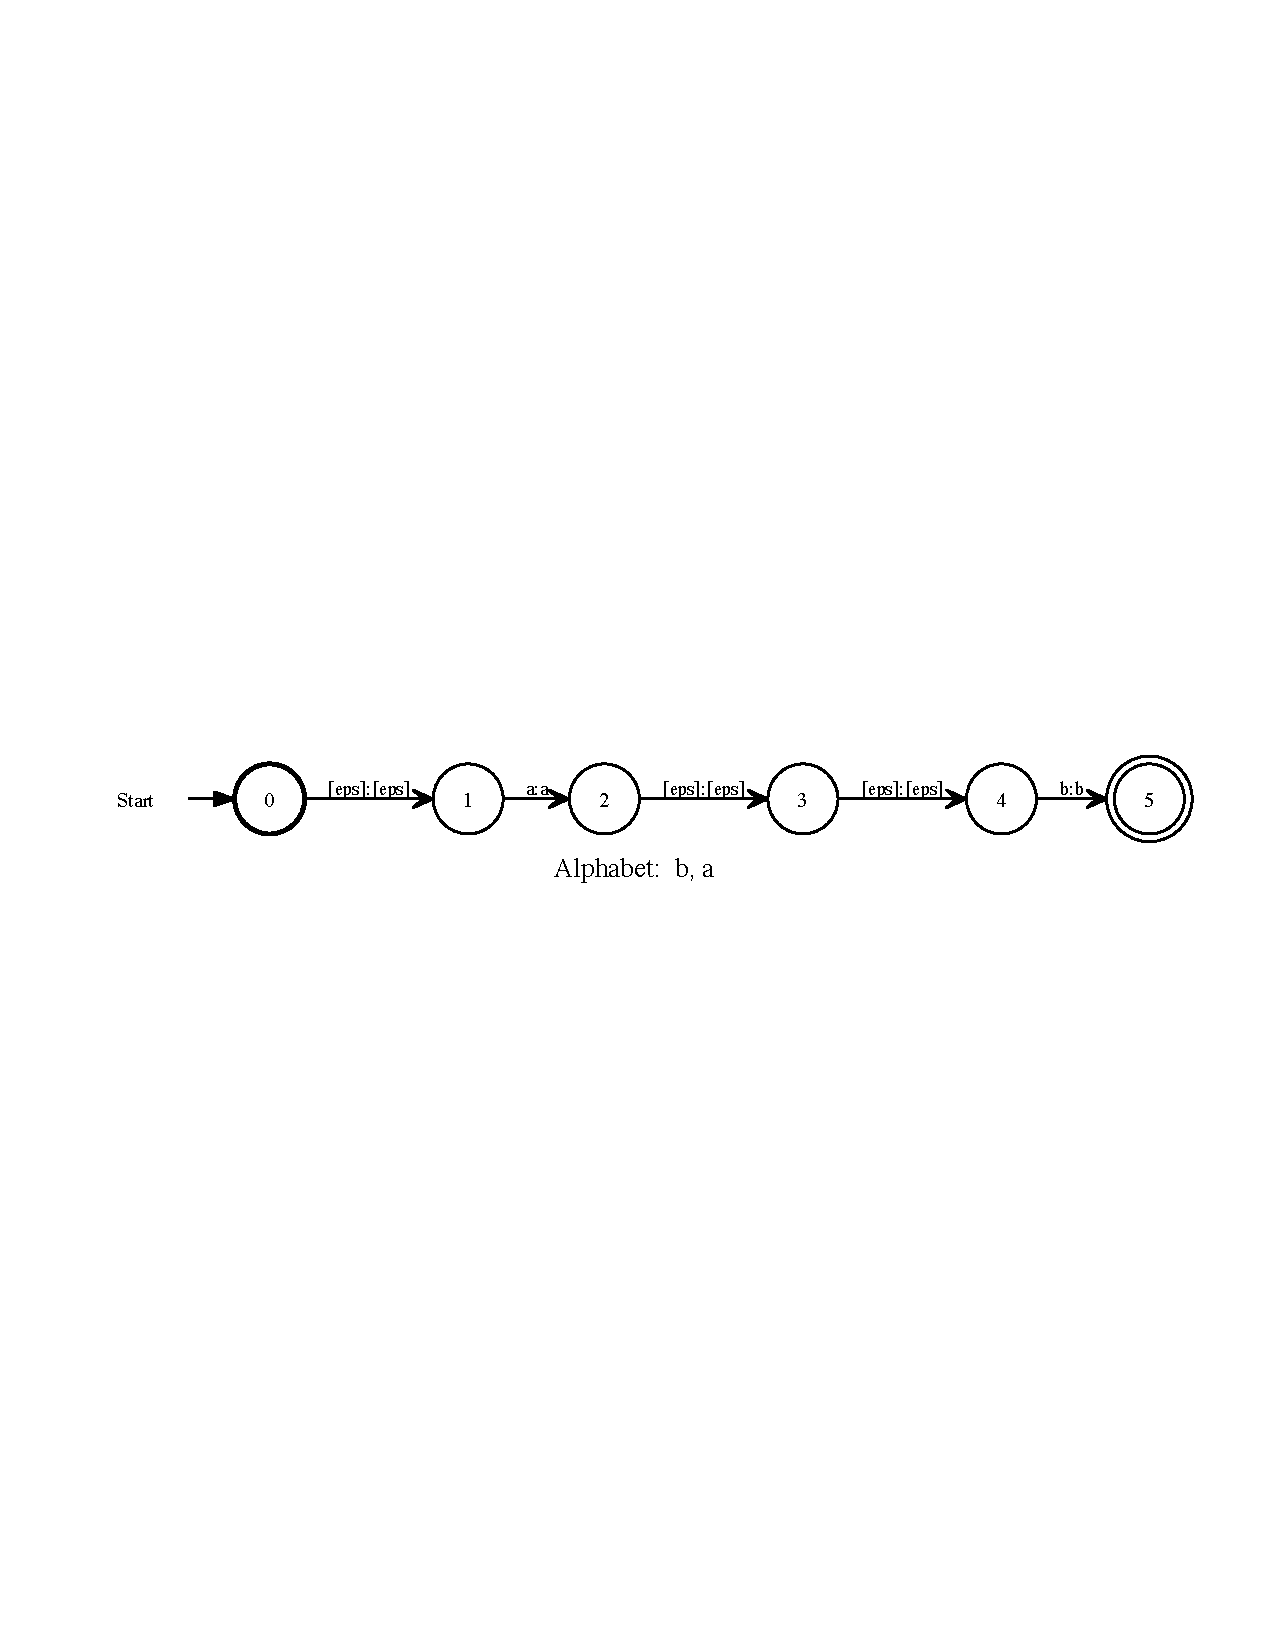
\includegraphics[width=135mm]{images/aEpsb.pdf}
%\includegraphics[scale=0.9]{images/<filename>.pdf}
%\includegraphics[width=60mm]{images/<filename>.pdf}
%\includegraphics[height=60mm]{images/<filename>.pdf}
\end{center}

\noindent
including the epsilon indicated by the regular expression, plus two other epsilons
introduced by the concatenation algorithm.  By default, however, the \fsm{}
is automatically epsilon-removed to produce the equivalent but more compact result

\begin{center}
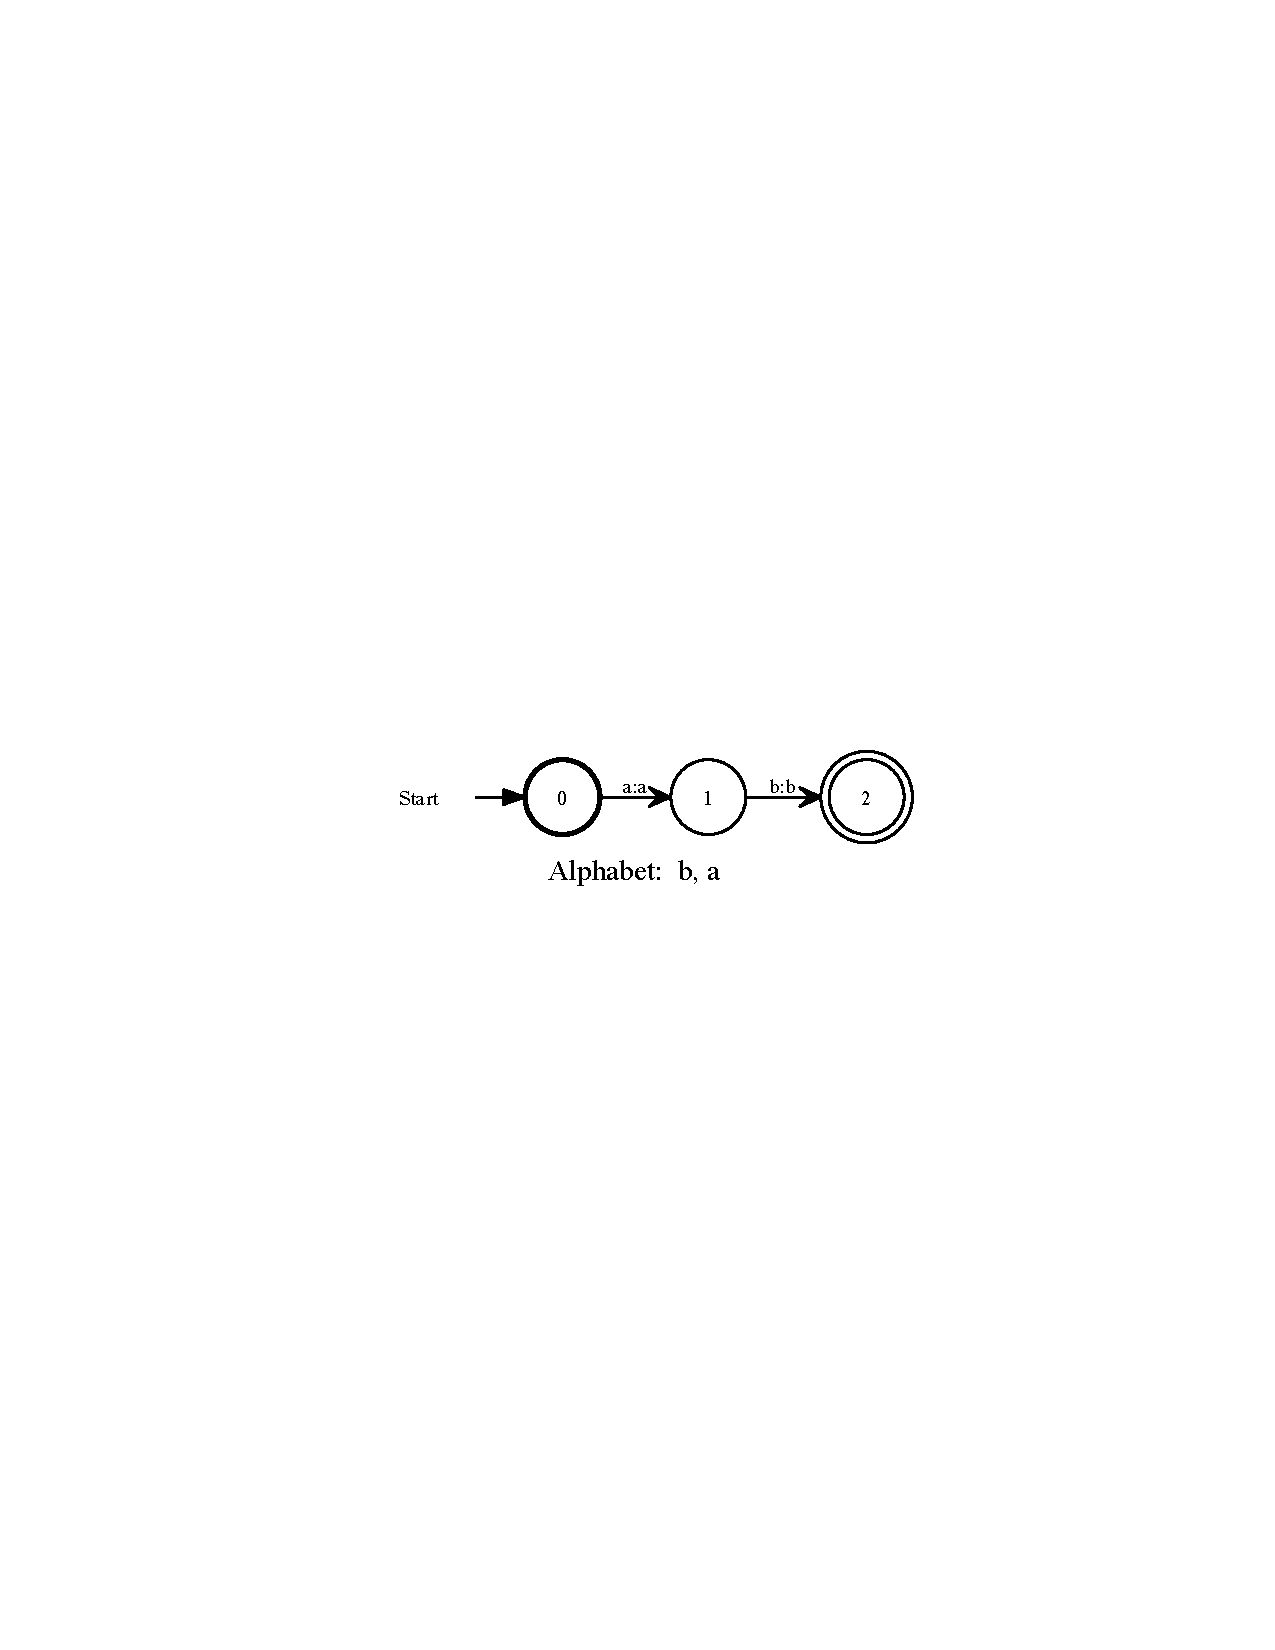
\includegraphics{images/aEpsbOptimized.pdf}
%\includegraphics[scale=0.9]{images/<filename>.pdf}
%\includegraphics[width=60mm]{images/<filename>.pdf}
%\includegraphics[height=60mm]{images/<filename>.pdf}
\end{center}

Consider also the following example, which has multiple words that start
with the same symbol(s) and multiple words that end with the same
symbol(s).


\begin{Verbatim}
$foo = rat | bat | rabbit | bird | cod ;
\end{Verbatim}

\noindent
The raw, unoptimized \fsm{} looks like this, including a number of
epsilon arcs:


\begin{center}
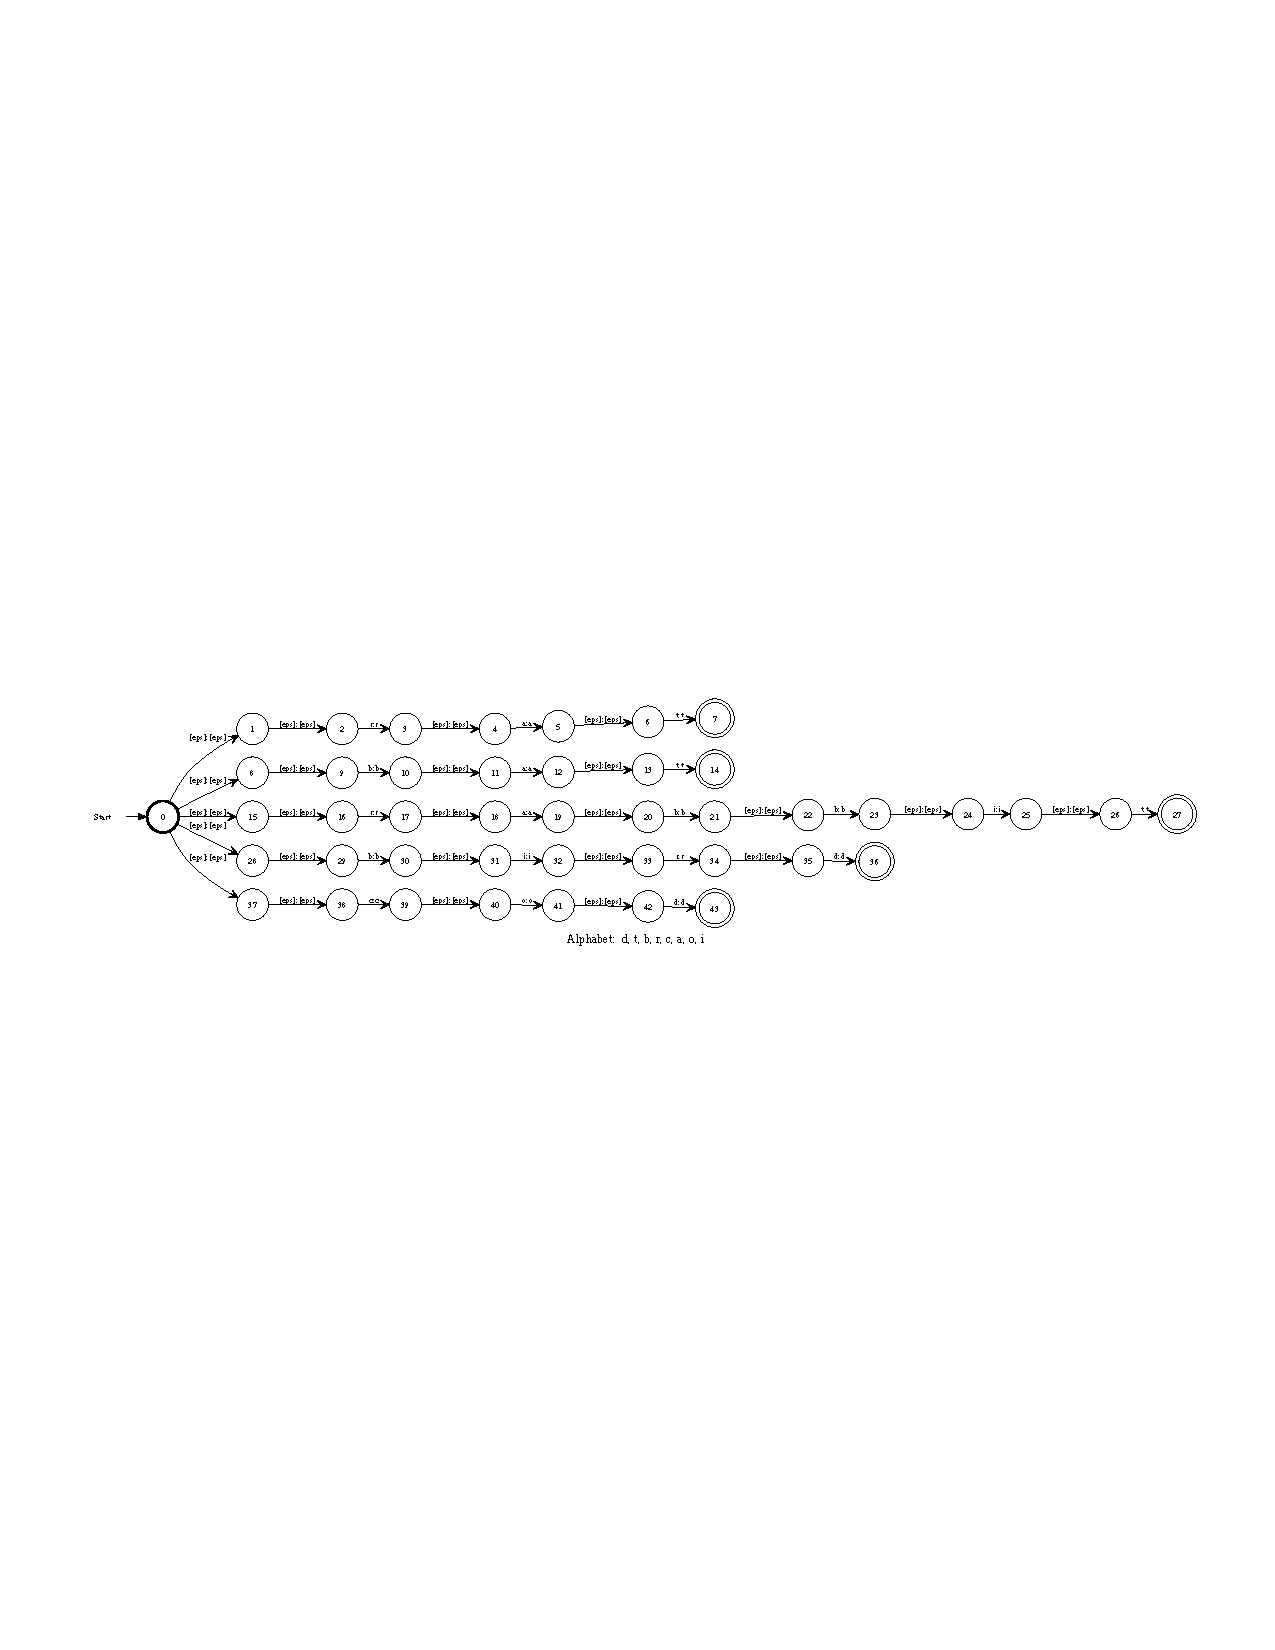
\includegraphics[width=135mm]{images/unoptimized.pdf}
%\includegraphics[scale=0.9]{images/<filename>.pdf}
%\includegraphics[width=60mm]{images/<filename>.pdf}
%\includegraphics[height=60mm]{images/<filename>.pdf}
\end{center}

\noindent
This machine accurately encodes the five-word language, but in a less than
optimal way.
Just by running epsilon-removal, the \fsm{} is considerably simplified,
resulting in the following machine:


\begin{center}
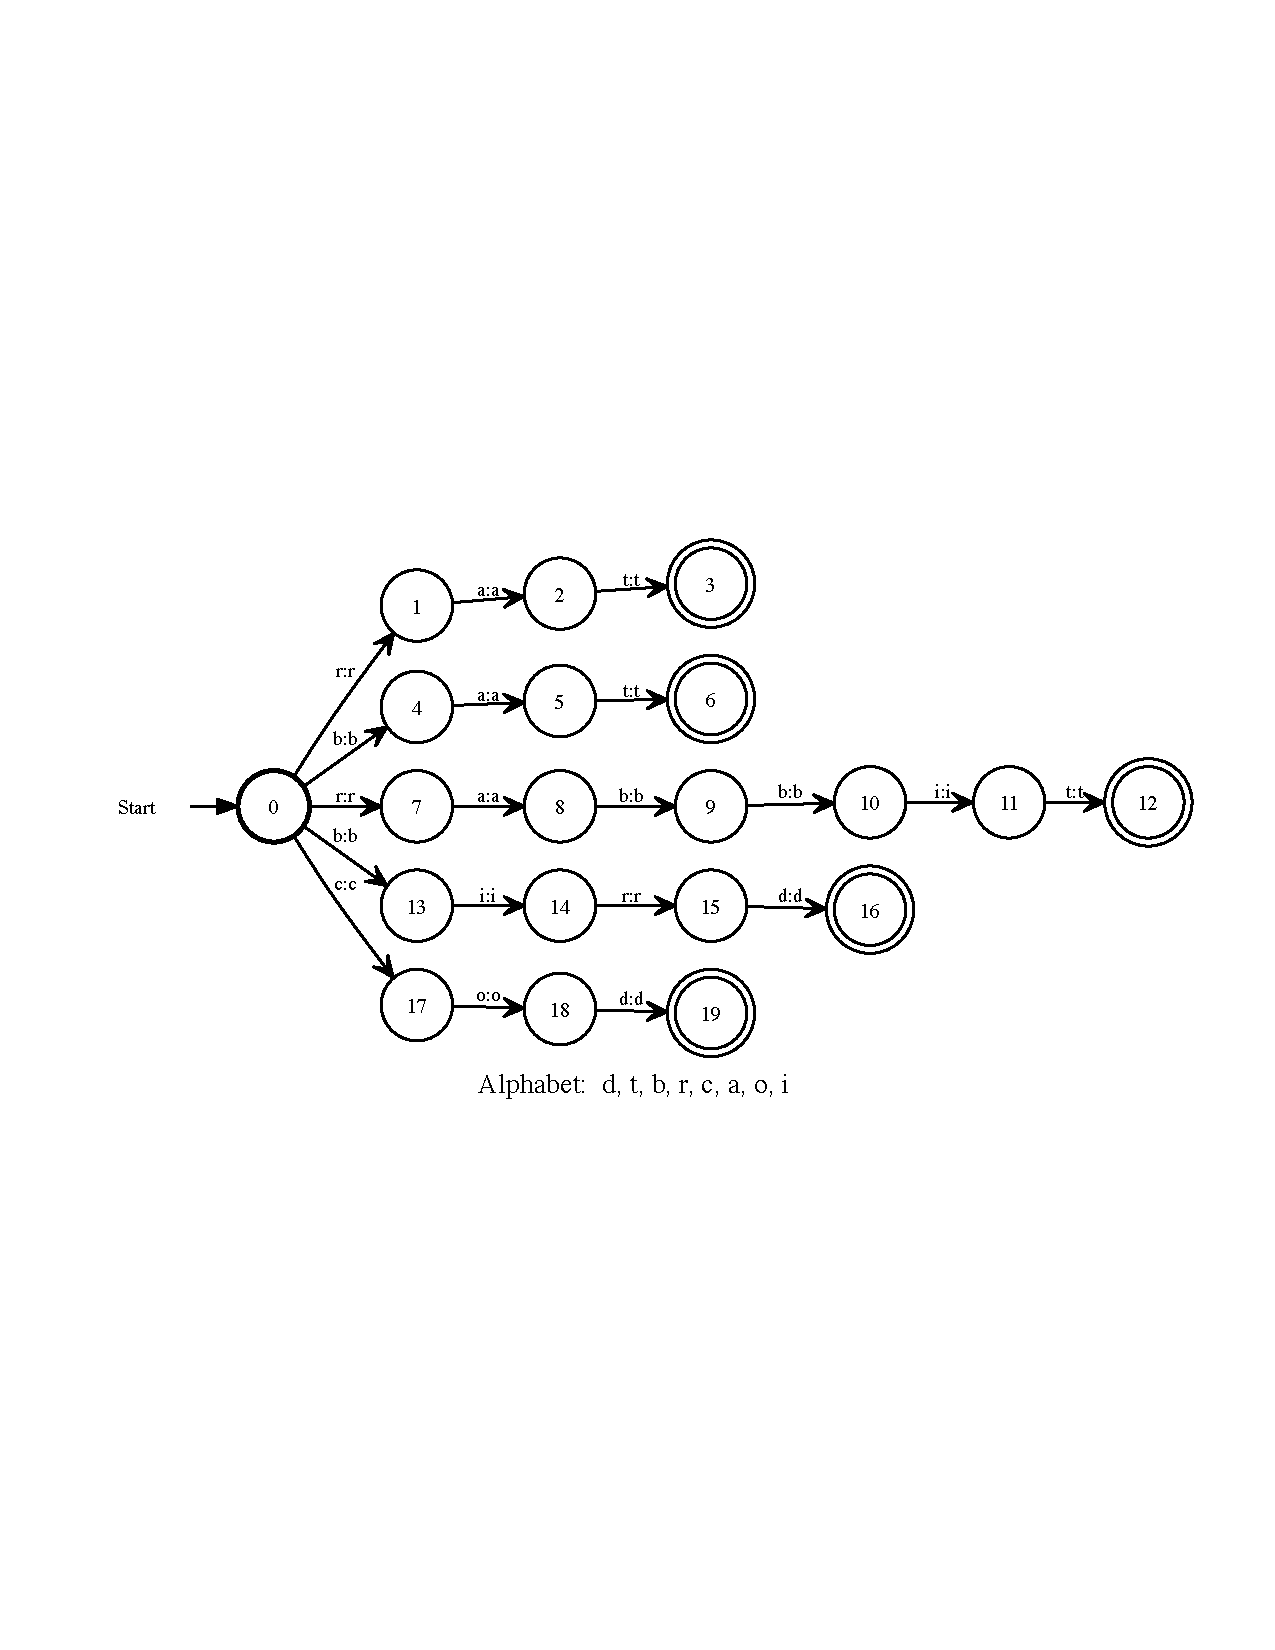
\includegraphics[width=135mm]{images/epsremoved.pdf}
%\includegraphics[scale=0.9]{images/<filename>.pdf}
%\includegraphics[width=60mm]{images/<filename>.pdf}
%\includegraphics[height=60mm]{images/<filename>.pdf}
\end{center}

\noindent
At this point, note that if you apply the machine to the input string
``rat,'' its operation is going to be \emph{non-determnistic}.  Starting in
the machine's start state, and placing the match pointer at the first input symbol
\texttt{r}, there are in fact two arcs labeled \texttt{r} exiting the start state, 
and both of these arcs will need to be
explored.  Of course, only one of them will result in a successful match, 
but time will be wasted
exploring the wrong \texttt{r}-labeled arc. 

The solution to the non-determinism problem is to \emph{determinize} the
\fsm{}, resulting in the following modified machine


\begin{center}
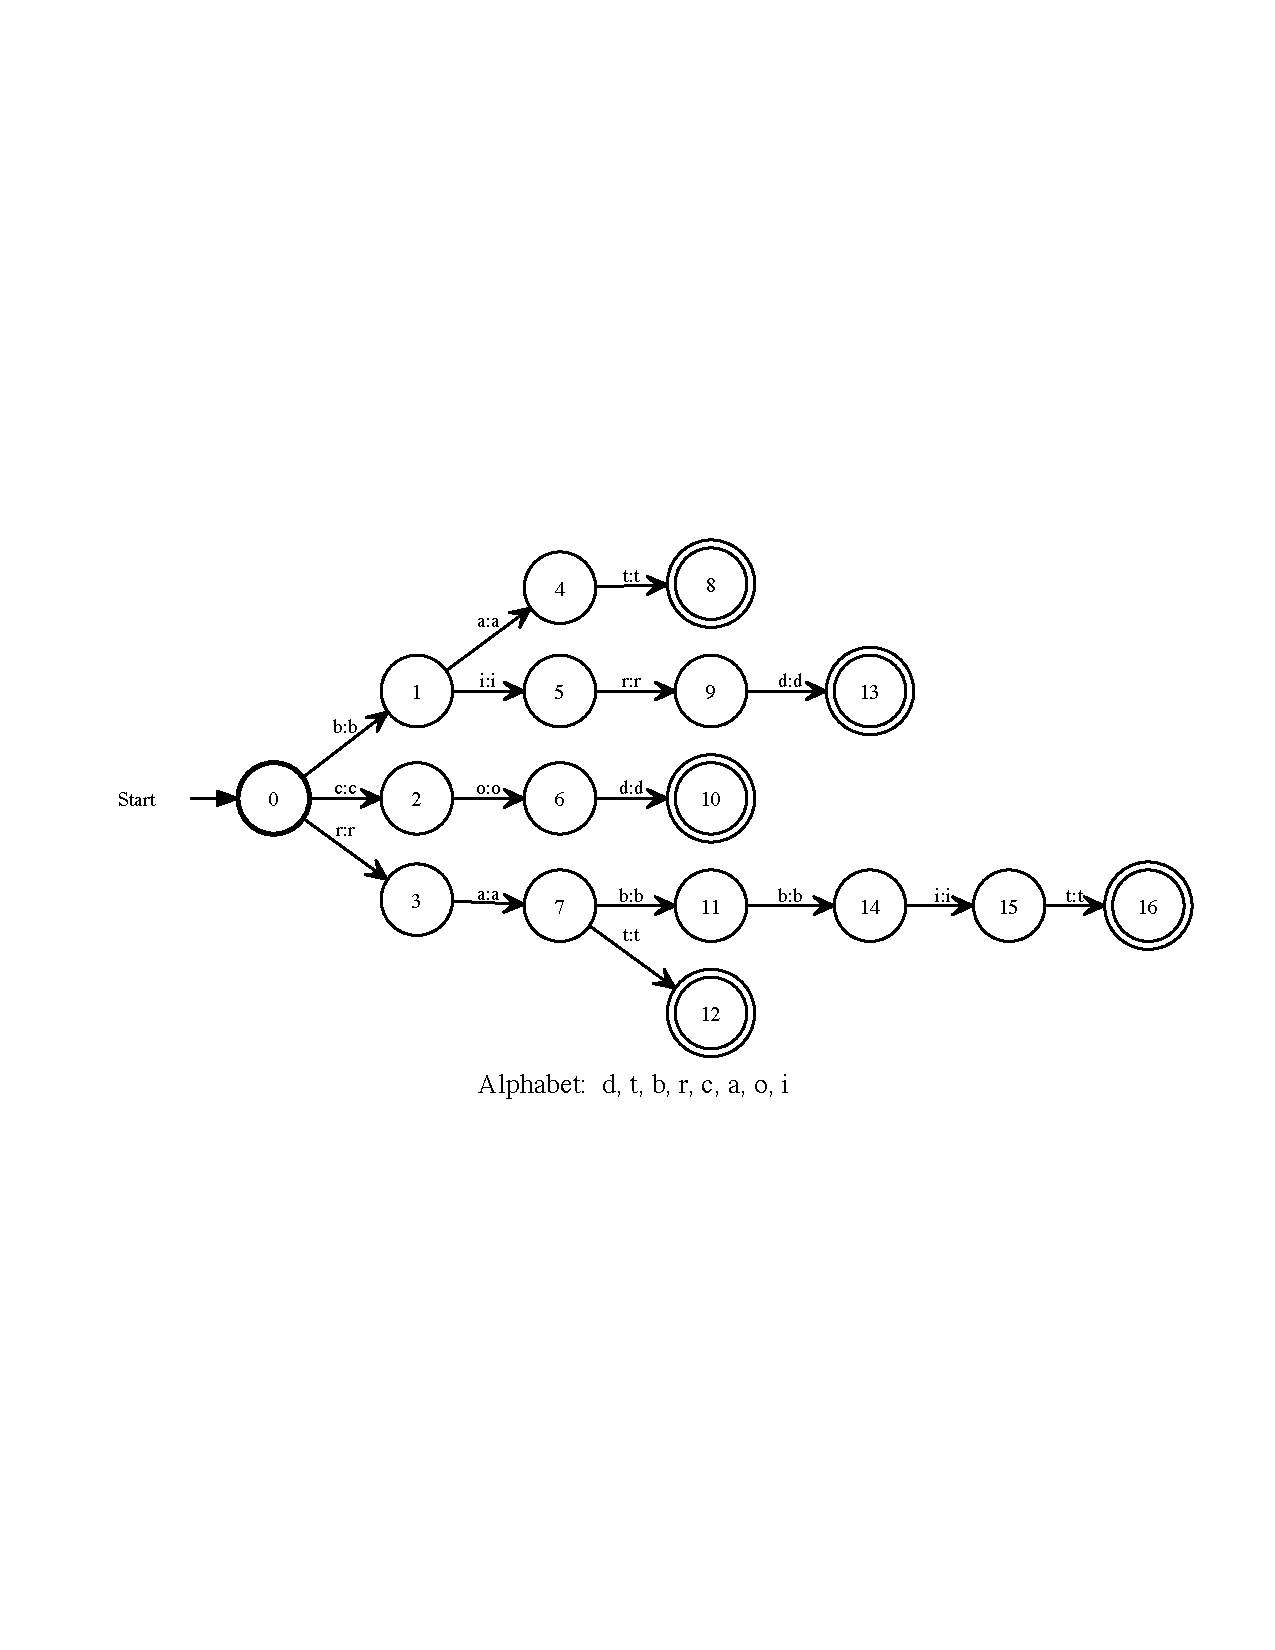
\includegraphics[width=135mm]{images/determinized.pdf}
%\includegraphics[scale=0.9]{images/<filename>.pdf}
%\includegraphics[width=60mm]{images/<filename>.pdf}
%\includegraphics[height=60mm]{images/<filename>.pdf}
\end{center}

\noindent
Note that the paths for the words ``rat'' and ''rabbit,'' which both start
with the prefix ``ra,'' now share the states and arcs for recognizing that
prefix.  When the determinized machine is applied to ``rat'' or ``rabbit,'' the
application algorithm no longer wastes time exploring the wrong path.  Note
also that the \texttt{b} prefix shared by ``bat'' and ``bird'' is also
represented in the machine by shared states and arcs.

At this point, we have a deterministic machine that can be applied to input
strings with maximum efficiency, but note that the machine itself is bigger
than it really needs to be.  In particular, note that ``rat,'' ``bat'' and
``rabbit'' all end with the same \texttt{t} suffix, but the \fsm{}
represents them with separate states and arcs.  The solution to this problem
is to \emph{minimize} the machine, resulting in this final optimal machine:


\begin{center}
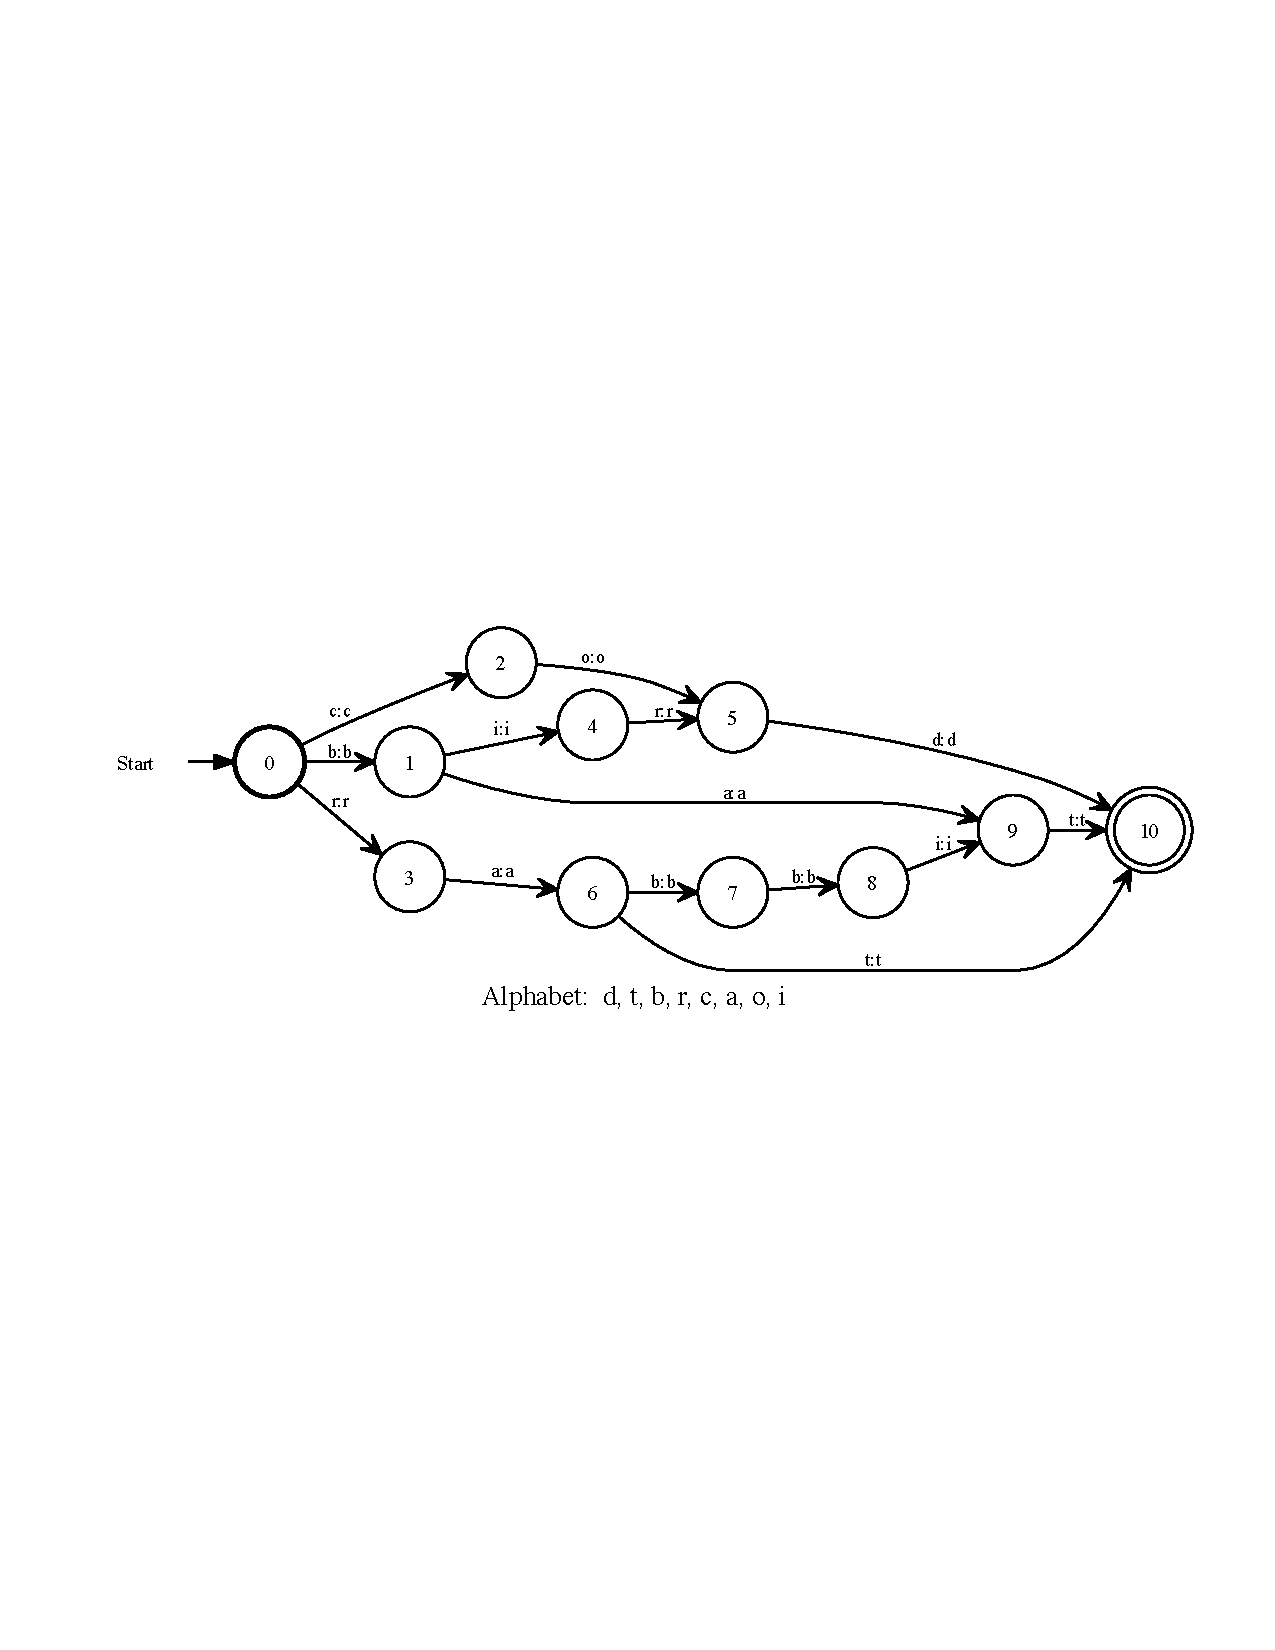
\includegraphics[width=135mm]{images/minimized.pdf}
%\includegraphics[scale=0.9]{images/<filename>.pdf}
%\includegraphics[width=60mm]{images/<filename>.pdf}
%\includegraphics[height=60mm]{images/<filename>.pdf}
\end{center}

As you will recall, we started with the superficially simple regular
expression


\begin{Verbatim}
$foo = rat|bat|rabbit|bird|cod ;
\end{Verbatim}

\noindent
At each stage shown, the \fsm{} encoded the same language of five words, but
as we epsilon-removed, determinized and minimized the machine, it became
both more efficient to apply, and smaller in its storage requirements.  In
real-life applications, where \fsm{}s can encode languages of millions of words, and the
machines can easily contain tens of thousands of states and arcs, and
runtime performance is critical, the
processes of epsilon-removal, determinization and minimization---known
collectively as \emph{optimization}---are vital.  Luckily, Kleene
automatically optimizes all \fsm{}s by default, and the average Kleene
programmer never has to worry about it.\footnote{Expert users may occasionally
want to turn off one or more of the optimization processes, and Kleene provides
a way to do this.  See Appendix \ref{app:optimize}.} 

\subsection{Using Defined Variables}

Once a variable has been bound to an \fsm{} value, it can be used in subsequent regular
expressions, e.g.

\begin{Verbatim}
$fsm1 = dog | cat | elephant ;
$fsm2 = horse | pig | sheep ;
$fsm = $fsm1 | $fsm2 ;
print $fsm ;
// outputs: dog cat elephant horse pig sheep
\end{Verbatim}


\subsection{Characters}

\subsubsection{Unicode}

Kleene supports the Unicode character set, 
which current contains over 100,000 defined characters and has a capacity
to encode over 1 million characters.  Programmers are encouraged to edit their Kleene scripts
directly in Unicode using their favorite Unicode-capable text editors, though Kleene 
can read and process scripts written in all common character sets.  

The Kleene \gui{} is written using the Java Swing library; its text widgets are
automatically Unicode-capable, and you can use standard Java input methods to facilitate
typing in exotic characters.  In some cases, it may be convenient to designate Unicode
characters by their code point value.  Unicode characters in the Basic Multilingual Plane
can all be encoded using four hexadecimal digits, and in Kleene regular expressions they
can be designated as the \acro{ascii} sequence \verb!\uHHHH!, where \texttt{H} is in the
set [0-9a-fA-F].\footnote{That is, each \texttt{H} can be a digit from 0 to 9 or a letter
from \texttt{A} to \texttt{F}, in either uppercase or lowercase.}  The following two
examples are equivalent,


\begin{Verbatim}
$fsm1 = a b c α β γ ;
$fsm2 = a b c \u03b1 \u03b2 \u03b3 ;
\end{Verbatim}

\noindent
because 03b1 (hexadecimal) is the code point value of the Greek alpha, 03b2 is the beta,
and 03b3 is the gamma.  Both expressions result in an \fsm{} that looks like


\begin{center}
\includegraphics[width=135mm]{images/alphabetagamma.pdf}
%\includegraphics[scale=0.9]{images/<filename>.pdf}
%\includegraphics[width=60mm]{images/<filename>.pdf}
%\includegraphics[height=60mm]{images/<filename>.pdf}
\end{center}

\noindent
In OpenFst (and Kleene) \fsm{}s, the labels on arcs are in fact integers,
and in Kleene these integers are Unicode code point values.  Where possible,
the code point values are displayed by the \texttt{draw} facility as
letters.  The Graphiviz \texttt{dot}
facility, which is used to display the \fsm{}s, has limitations in displaying characters
like α, β and γ, so they are displayed in hexadecimal.  

Kleene can also handle Unicode supplementary characters, and they can be entered as the
\acro{ascii} sequence
\verb!\uHHHHHHHH!, that is, \verb!\u! followed by exactly eight hexadecimal digits.  The following
example contains the first three characters in the Deseret Alphabet, which is encoded in
the supplementary area.


\begin{Verbatim}
$fsm = \U00010400 \U00010401 \U00010402 ;
draw $fsm ;
\end{Verbatim}

\noindent
This results in the following \fsm


\begin{center}
\includegraphics[width=135mm]{images/desalph.pdf}
%\includegraphics[scale=0.9]{images/<filename>.pdf}
%\includegraphics[width=60mm]{images/<filename>.pdf}
%\includegraphics[height=60mm]{images/<filename>.pdf}
\end{center}

\noindent
which has a single supplementary code point value on each arc.\footnote{However, if the
characters are entered in a Swing text widget using the Java CodePoint Input Method, each
character is somehow divided into the two \init{bmp} surrogate characters used to encode
the single supplementary character in the UTF-16 encoding.  This behavior needs to be
reviewed in the context of Kleene.}



\subsubsection{Multi-character Symbols}

In addition to Unicode characters, it is often useful to have user-defined symbols that
have multi-character names, often called ``multi-character symbols.''  For example, you can
define [Noun], [Verb], [Adj], [Adv], [Sing], [Plur], etc.\@ as symbols that suggest
linguistic categories or features.  In another notational tradition, these might be spelled +Noun,
+Verb, +Adj, etc.  In Kleene syntax, you simply surround a string of characters in single quotes
to indicate that they are to be treated as a single multi-character symbol.


\begin{Verbatim}
$fsm = a b '[Noun]' ;
\end{Verbatim}

\noindent
The single quotes delimit the name of the symbol but are not actually part of the symbol
name.  Each multi-character symbol is also stored as an integer label on an arc in the result
\fsm{}, and the integer is taken from a Unicode Private Use Area (\init{pua}).

In general it is recommended that multi-character symbol names include at least
one punctuation character to help human beings distinguish them from sequences of
alphabetical characters.  There is nothing to prevent you from using a
multi-character symbol like \texttt{noun}, by putting \verb!'noun'! in a regular
expression,


\begin{Verbatim}
// a multi-character symbol without punctuation, NOT recommended
$myfsm = 'noun' ;
print $myfsm ;
// outputs: noun

// a concatenation of four symbols
$yourfsm = noun ;
// outputs: noun
\end{Verbatim}

\noindent
but the printed output \texttt{noun}, being a single multi-character symbol,
is humanly indistinguishable from the printed word ``noun''
that is a concatenation of four separate symbols.  In practice, the use of
multi-characters symbols like \verb'noun' leads to much confusion and is
strongly discouraged.  

\subsubsection{Characters in Variable Names}

\fsm{} variable names in Kleene start with a dollar sign, a letter, and then any number of
letters and digits.


\begin{Verbatim}
$fsm = a b c ;
$fsm1 = x y z ;
$q7 = r s t ;
\end{Verbatim}

\noindent
The letters after the dollar sign can include any letters in the Unicode \init{bmp} (Basic
Multilingual Plane).\footnote{Because of limitations in JavaCC and Java itself, variable
names cannot contain supplementary characters.}  The following two assignments are equivalent 


\begin{Verbatim}
$αβ = a b ;
$\u03b1\u03b2 = a b ;
\end{Verbatim}

Kleene supports Unicode to the extent that Java does, which is pretty well but not
perfectly.  Users can write their scripts using the International Phonetic Alphabet, Greek,
Cyrillic, Arabic, etc.\@ without ever needing to resort to clumsy transliterations.
Whether the Kleene \gui{} can actually display a character depends on the fonts installed in
your Java installation.

\subsection{Regular Languages and Regular Relations}

\subsubsection{Regular Languages and Acceptors}

In formal language theory, a language is a set of strings.  A regular language, where
\emph{regular} is a technical term,\footnote{In some traditions, the term
\emph{rational} is used instead of \emph{regular}.} is formally defined as a language that can be defined
using only concatenation, union and the Kleene-closure\footnote{The Kleene-closure is named
after mathematician Steven Cole Kleene, who invented it.  The Kleene programming language
is named after the same man.} operator *, which indicates zero or
more repetitions.  Any finite (i.e.\@ not infinite) language is a regular language.  Some infinite languages,
such as \verb!b*!, which is the language of all strings that contain zero or more
\texttt{b} letters, are also regular.  Some infinite languages are not regular
and so cannot be encoded in an \fsm{}; we cannot handle such languages in Kleene.

A regular language can be encoded as an \fsm{} (Finite-State Machine) called an
\emph{acceptor}.  An \fsm{} has a finite number of states, one of which is designated as the
start state, and zero or more of which are final.  An \fsm{} can also contain zero or
more labeled directed arcs that lead from a state to a state.

When an acceptor is applied to an input string, it will either accept it or reject it.  It
will accept all and only the strings in the regular language that it encodes.

In classic visualizations of acceptors, they have only a single label on
each arc.  In OpenFst, and therefore in Kleene, all arc labels have two labels, an input
label and an output label: \verb!i:o!.  By convention in OpenFst, an \fsm{} is an acceptor,
or can be interpreted as an acceptor,
if and only if each input label is equal to its associated output label.

Regular languages, and the acceptors that encode them, have some very interesting and
useful
mathematical properties, known as closure properties.  For example, regular languages are
\emph{closed} under the union operation because if you union any two regular languages together, the
result is also a regular language.  Regular languages and the acceptors that
encode them are closed under the following
operations:

\vspace{4mm}

\begin{tabular}{|l|l|}
\hline
Concatenation 	& A B \\
\hline
Union         	& A | B \\
\hline
Iteration	  	& A*\\
\hline
Subtraction		& A - B\\
\hline
Intersection	& A \& B\\
\hline
Complementation		& \~{}A\\
\hline
\end{tabular}

\subsubsection{Regular Relations and Transducers}

Whereas a regular \emph{language} is a set of strings, a regular \emph{relation}
is a set of
\emph{ordered pairs}
of strings.  For example, (dog, dogs), (cat, cats), (elephant, elephants), (woman, women)
and (deer, deer)
are ordered pairs of words that, in English, have a singular noun as the first word, and its plural
as the second word.  A set of such pairs, denoted in set theory (not Kleene syntax) as \{ (dog, dogs), (cat, cats), (elephant,
elephants), (woman, women), (deer, deer) \}, is a regular relation.  All finite relations are
regular relations.  Some infinite relations are also regular.

A regular relation can be encoded as an \fsm{} called a \emph{transducer}.  Theoretically,
regular relations and finite-state transducers can have any number of levels, known as
\emph{projections}, but OpenFst and most practical computer implementations have been limited to two.
A finite-state transducer (\fst{}) has a finite number of states, one of which is
designated as the start state, and zero or more of which are final.  An \fst{} can also
contain zero of more labeled directed arcs that lead from a state to a state.  Each label
consists of two parts, an input label and an output label, notated  \verb!i:o!.  In a finite-state
transducer, the input
and output labels of an arc can be different, or the same.

In Kleene syntax, a label with \texttt{a} on the input side and \texttt{b} on the output
side is denoted \texttt{a:b}.  The statement


\begin{Verbatim}
$fsm = a:b ;
\end{Verbatim}

\noindent
results in the \fst{}


\begin{center}
\includegraphics{images/aoverb.pdf}
%\includegraphics[scale=0.9]{images/<filename>.pdf}
%\includegraphics[width=60mm]{images/<filename>.pdf}
%\includegraphics[height=60mm]{images/<filename>.pdf}
\end{center}


\noindent
More generally, : is the \emph{cross-product} operator that takes two operands that must
both denote regular languages (not regular relations).  It creates a regular relation with the
left operand as the input projection, and the right operand as the output projection.
Often the cross-product operator is used to map
individual strings, as in this example.


\begin{Verbatim}
$fsm = (dog):(dogs) | (cat):(cats) | (elephant):(elephants) |
       (woman):(women) | (deer):(deer) |
       (formula):(formulas) | (formula):(formulae) ;
\end{Verbatim}


More generally, the operands of the cross-product operator : can denote arbitrarily complex regular languages, 
and every string in the input language is related to every string of the
output language, and vice-versa.  Consider, for example,

\begin{Verbatim}
$foo = (dog|cat|rat):(animal|mammal) ;
\end{Verbatim}

\noindent
where the input (upper-side) language consists of the strings ``dog,'' ``cat'' and ``rat,'' and the output (lower-side)
language consists of the strings ``animal'' and ``mammal.''  The cross-product is an \fst{} that
relates ``dog'' in the input language to both ``animal'' and ''mammal'' in the output
language.  And similarly for ``cat'' and ``rat.''  The resulting relation
contains the six ordered pairs (dog, animal), (dog, mammal), (cat, animal), (cat,
mammal), (rat, animal) and (rat, mammal).  Note that a relation is a set of ordered string
pairs, and the order of the string pairs is not significant.

\subsubsection{Applying Transducers}

In the OpenFst visualization, an \fst{} is \emph{applied} to an input string by
matching the symbols of the input string against a sequence of \emph{input symbols}.  If the input string matches successfully
and completely against a sequence of input symbols, on a \emph{path} leading from the start state,
arc-by-arc to a final state, 
the output is a string consisting of the sequence of \emph{output symbols} from the same path 
in the \fst{}.  

The output string can be different from the input string, and thus
the \fst{} can \emph{transduce} or \emph{map} from one kind of string to another kind of string.  To return to the
previous noun example, if an ordered pair (dog, dogs) is interpreted as (\emph{inputString},
\emph{outputString}),
then the \fst{} that encodes the regular relation { (dog, dogs), (cat, cats), (elephant,
elephants), (woman, women), (deer, deer)} would provide a transduction or \emph{mapping}
from singular nouns like ``dog,'' ``cat'' and ``woman'' to their \emph{related} plural forms ``dogs,''
``cats'' and ``women,'' respectively.  Relations relate words to other words. 
Looked at in the other direction,
the same \fst{} provides a mapping from plural forms to their
related singular forms.

Try building and testing the following example in the Kleene \gui{}:


\begin{Verbatim}
$numberMapper = (dog):(dogs) | (cat):(cats) | 
      (elephant):(elephants) | (woman):(women) | (deer):(deer) |
      (formula):(formulas) | (formula):(formulae) |
      (cherub):(cherubim) | (man):(men) | (knife):(knives) ;
test $numberMapper ;
\end{Verbatim}

\noindent
Enter a singular noun like ``dog'' in the upper-side input field, and the output
will be the plural form ``dogs.''  Enter ``formula'' in the upper-side input
field, and the output will be the two plural forms:  ``formulas'' and
``formulae.''  


An \fsm{} encoding an acceptor can also be interpreted and used as an \emph{identity transducer}
that maps each of the words in the language to itself.

An \fst{} that encodes a relation is \emph{functional} if each input string has exactly one
output string.  Very commonly when modeling natural languages, an \fst{} can map one input
string to multiple output strings, reflecting ambiguity. 

A regular relation is a relation between two regular languages, one of which is, in the
OpenFst tradition, termed the
\emph{input projection} and the other the \emph{output projection}.  In all cases, every
string in the input language/projection is related to at least one
string in the output language/projection, and each string in the output language/projection is related to at
least one string in the input language/projection.

In the Xerox
visualization of \fst{}s, which emphasizes the bi-directionality of \fst{s}, the projections
are called \emph{upper} and \emph{lower} rather than \emph{input} and \emph{output}.  
What OpenFst calls normal application, matching the symbols
of an input string against ``input'' symbols on a path, outputting the corresponding
``output'' symbols, Xerox calls \emph{generation} or ``application in a downward
direction,'' matching the symbols of the input string against upper-side labels, and
outputting strings of lower-side labels.  Xerox
researchers also talk about \emph{analysis} or ``application in an upward direction,'' matching the symbols of
the input string against lower-side symbols, and outputting strings of upper-side symbols.  

The following transducer, which includes multi-character symbols,
models the formation of regular English plurals more elegantly, and illustrates the Xerox
visualization.

\begin{Verbatim}
// a set of noun roots
$nroot = dog|cat|bird|horse|worm ;
$ncat = '[Noun]':"" ; // [Noun] tag on the upper side,
                      // the empty string on the lower side
$num = '[Sg]':"" | '[Pl]':s	; 
// [Sg] on the upper side, 
//   and empty string on the lower.
// [Pl] on the upper side, 
//   and s on the lower

// now just concatenate the three FSMs
$nouns = $nroot $ncat $num ;

test $nouns ; // and launch the test window
\end{Verbatim}

\noindent
The resulting \fst{} looks like this:

\begin{center}
\includegraphics[width=135mm]{images/simplenounsgpl.pdf}
%\includegraphics[scale=0.9]{images/<filename>.pdf}
%\includegraphics[width=60mm]{images/<filename>.pdf}
%\includegraphics[height=60mm]{images/<filename>.pdf}
\end{center}


\noindent
showing that strings like ``dog[Noun][Sg]'' and ``cat[Noun][Pl]'' are in the upper-side
language, while their related strings like ``dog'' and ``cats'' are in the lower-side language. 
The \texttt[eps] character in the diagram represents the empty-string language, called the
\emph{epsilon} by convention.
When you \texttt{test} the network and enter \texttt{cat[Noun][Pl]} in the \emph{upper}-side
entry field, the output is 

\begin{Verbatim}
cats: 0.0
\end{Verbatim}

\noindent
Again, just ignore the weight \texttt{0.0}, which will be explained later.  If you enter
\texttt{horse[Noun][Sg]} in the upper entry field, the output will be \texttt{horse}.  Xerox
researchers working on morphology 
generally referred to this kind of application as \emph{generation}, taking
an abstract upper-side string and generating a surfacy lower-side string (or strings).  Now,
applying the same \fst{} in the opposite direction, try entering 
\texttt{horse} in the \emph{lower} input field; the result will be \texttt{horse[Noun][Sg]}.
And if you enter \texttt{horses} in the lower input field, the output will be \texttt{horse[Noun][Pl]}.
Xerox researchers referred to this mode of application as \emph{analysis}, mapping from surfacy
strings to abstract analysis strings.  \fst{}s are bidirectional, and the Xerox visualization of
\fst{}s emphasizes that bidirectionality. 
Such \fst{}s, which perform morphological analysis and
generation, can be written to model word analysis in natural languages like English, French, German,
Arabic, Zulu, etc.

As we shall see, there is value to both the Xerox and the OpenFst
visualizations of \fst{}s.   Although, as the Xerox tradition emphasizes,
an \fst{} can always be applied validly in either
direction, downward or upward, a determinization algorithm cannot
generally determinize both sides of an \fst{}---it has to
determinize one side or the other.\footnote{In some traditions, the term
\emph{determinization} is used for acceptors, and the determinization of one
side of a transducer is called \emph{sequentialization}.}  The OpenFst determinization
algorithm optimizes what the OpenFst tradition calls the input side, and
because the input side is determinized, and the output side is not necessarily determinized at the same time, 
it is generally more efficient to match
input strings against the input side than against the output side. 

In Kleene, one is free to build \fst{}s in any orientation that the
programmer finds intuitive.  But one should be aware that it is always
the upper side---what OpenFst calls the input side---that is determinized
for the most efficient runtime application.  If you intend to apply
	your  \fst{} in a downward direction, matching input against the
	upper side, and reading the results off the lower side, then it is
	already in the proper orientation for the most efficient operation.  
	
If, however, you build an \fst{}
that is properly applied in an upward direction, matching the input
against the lower side, to get the results you need, all you have to do,
as a final step, is to \emph{invert} the \fst{}.  Inversion exchanges the upper
side and the lower side, such that the new upper side (the old lower
side) will be determinized for the most efficient application.  Then use
the inverted \fst{} in the OpenFst way, matching input strings against the
new ``input'' side.

In Kleene, some operations like inversion are implemented as pre-defined
functions rather than using operators.  Here is how you take a defined
\fst{} and compute its inversion.

\begin{Verbatim}
$invertedFst = $^invert($fst) ;
\end{Verbatim}

\noindent
That is, Kleene provides a function named \verb!$^invert! that takes one argument, an \fst, and
returns a new \fst{} that is the inversion of the argument.  The argument itself is not modified. 

\subsubsection{Closure Properties of Regular Relations/Transducers}

The closure properties of regular relations, and of the \fst{}s that encode them, are not
the same as the closure properties of regular languages.  In particular, \fst{}s are closed
under concatenation, union and iteration, but not generally under subtraction, intersection
or complementation.

\vspace{4mm}

\begin{tabular}{|l|l|}
\hline
Concatenation 	& A B \\
\hline
Union         	& A | B \\
\hline
Iteration	  	& A*\\
\hline
\end{tabular}

\vspace{4mm}

\noindent
If you try to subtract, intersect or complement transducers, Kleene will
throw an exception and you will get an error message.
The illegal operations for transducers all reduce to subtraction.

\vspace{4mm}

\begin{tabular}{|l|l|}
\hline
Operation & Equivalent to \\
\hline
A - B  &  A - B \\
A \& B  &  A - (B - A)\\
\~{}A   &  .* - A\\
\hline
\end{tabular}

\subsubsection{Playing with \fst{}s}

A regular relation, encoded as an \fst{}, is a relation between two regular languages,
called the input projection and the output projection, and we can extract those
projections using the pre-defined Kleene functions \verb!$^inputProj()!
and \verb!$^outputProj()!.


\begin{Verbatim}
$fst = (dog|cat|rat):(animal|mammal) ;
$inputLang = $^inputProj($fst) ;
print $inputLang ;
// outputs: dog cat rat

$outputLang = $^outputProj($fst) ;
print $outputLang ;
// outputs: animal mammal
\end{Verbatim}

We can compute the inversion of an \fst{} with the \verb!$^invert()!
function, and the reverse of an \fsm{} (which reverses all the paths right-to-left)
with the \verb!$^reverse()! function.


\begin{Verbatim}
$fstinv = $^invert($fst) ;
$fstrev = $^reverse($fst) ;
\end{Verbatim}

\noindent
There are many more pre-defined functions in Kleene, and it is also possible to define your own functions.

Although you cannot, as we have already stated, subtract, intersect or complement
transducers, you can combine them using \emph{composition}, a powerful operation that we
will be exploring throughout the book.
In particular, composition is central to the application of \emph{alternation rules}, of
which Kleene offers a rich variety.  As a simple example, consider the rule

\begin{Verbatim}
$rule =  s -> z / (a|e|i|o|u) _ (a|e|i|o|u) ;
\end{Verbatim}

\noindent
or the equivalent

\begin{Verbatim}
$rule =  s -> z / [aeiou] _ [aeiou] ;
\end{Verbatim}

\noindent
which states that an \texttt{s} on the input side is mapped to a \texttt{z} on the output
side when it appears between two vowels.  The rule compiles into a transducer, which you can
draw and test in the usual ways:

\begin{Verbatim}
draw $rule ;
test $rule ;
\end{Verbatim}

\noindent
When you test \verb!$rule! and enter ``casa'' in the upper field, the output will be ``caza.''  If you input
``susisesos,'' the output will be ``suzizezos,'' mapping each input \texttt{s} into \texttt{z} only when it
appears between vowels.


\section{Looking at \fsm{}s}

As you build \fsm{}s, you will often want to see what they contain and what they look like. 
For finite (very finite) acceptors, you can print out the words in the regular language.


\begin{Verbatim}
$acc = (dog|cat|rat) s? ;
print $acc ;
\end{Verbatim}

\noindent
But printing out an infinite language is obviously out of the question, and Kleene will print
a warning if you try.  Even if a language
is infinite, the \fsm{} encoding it can still be small, as in

\begin{Verbatim}
$infLang = a* b* ;
draw $infLang ;
\end{Verbatim}

\noindent
and it can still be drawn.

In any non-trivial project, however, the \fsm{}s can soon become huge, consisting of hundreds of
thousands of states and arcs, and drawing is obviously out of the question.  In such cases,
one can still need to ask ``What do the input (or output) strings look like?'', and Kleene
offers some useful commands to show you random samples of the languages.  
In particular, the \texttt{randInput} command will print out
a random list of the input (upper-side) strings:

\begin{Verbatim}
randInput $fsm ;
\end{Verbatim}

\noindent
and \texttt{randOutput} will print out a random list of the output (lower-side) strings:

\begin{Verbatim}
randOutput $fsm ;
\end{Verbatim}

\section{Applications}

While it may be hard to imagine now, \fsm{}s can be used to implement a number of useful
applications for natural-language processing, including

\begin{itemize}
\item
Tokenizers
\item
Spelling checkers
\item
Spelling correctors
\item
Phonological models
\item
Morphological analyzer/generators
\item
Taggers (part-of-speech disambiguators)
\item
Shallow parsers
\item
Speech generator/recognizers
\end{itemize}

We have seen that \fst{}s can map an input string to a very different output string.  If
the input string is a normal English sentence, then the output string might be the same
string with token delimiters added---that would be a tokenizer.  We have seen that an
acceptor will accept all and only the strings in the language that it encodes.  If we then
had a large acceptor that encoded millions of strings that looked like properly spelled Spanish words, then
it would be the basis for a Spanish spelling checker, accepting Spanish words and rejecting
everything else.  Properly constructed \fst{}s could also map misspelled words into properly
spelled words, orthographical words into
strings of International Phonetic Alphabet symbols representing their pronunciation,
perhaps to be fed to a speech synthesizer, and
morphological analyzer \fst{s} would map orthographical words into analysis strings showing
the baseform, part of speech and other relevant information.  Such morphological analyzers
could be used to aid in dictionary lookup and to provide output to syntactic parsers.

Grammars consisting of multiple sub-components, performing tokenization, morphological
analysis, disambiguation and shallow-robust parsing can be written as \fst{}s and then
composed together into a single transducer that performs all the operations cleanly and
efficiently.  Speech synthesis and speech recognition are often approached this way.

This book will focus mostly on morphological analysis, which is often the first step in
computational linguistics.  After traditional fieldwork has defined the phonology,
morphology and orthography of a language, and after reasonable lexicography has been done,
a finite-state implementation like Kleene can help the linguist take that information, often paper-bound,
and animate it on
computers, creating
applications that analyze and look up words, providing a foundation for language
documentation, teaching, promotion and further computational linguistics.  The resulting
morphological analyzer can easily and repeated be tested, using millions of words, to
test its coverage and accuracy.  The writing of a finite-state
morphological
analyzer for a new language is a suitable and  popular project for a Master's thesis.


